\documentclass{article}


% if you need to pass options to natbib, use, e.g.:
%     \PassOptionsToPackage{numbers, compress}{natbib}
% before loading neurips_2024


% ready for submission
\usepackage[final]{neurips_2024}
\usepackage{xeCJK}\setCJKmainfont{IPAexMincho}% Xelatexで日本語を扱うためのパッケージ
\usepackage{algorithm,algpseudocode}% アルゴリズム

\usepackage[utf8]{inputenc}
\usepackage[T1]{fontenc}
\usepackage{amsmath}
\usepackage{amsfonts}
\usepackage{amssymb}
\usepackage[version=4]{mhchem}
\usepackage{stmaryrd}
\usepackage{graphicx}
\usepackage[export]{adjustbox}
\graphicspath{ {./images/} }
\usepackage{caption}
\usepackage{hyperref}
\hypersetup{colorlinks=true, linkcolor=blue, filecolor=magenta, urlcolor=cyan,}
\urlstyle{same}
\usepackage{bbold}

\title{Visual Autoregressive Modeling: Scalable Image Generation via Next-Scale Prediction }

\author{%
  Keyu Tian\textsuperscript{1,2}\thanks{Equal contribution.} \\
  \And
  Yi Jiang\textsuperscript{2}\textsuperscript{\dag} \\
  \And
  Zehuan Yuan\textsuperscript{2}\thanks{Corresponding author.} \\
  \And
  Bingyue Peng\textsuperscript{2} \\
  \And
  Liwei Wang\textsuperscript{1}\textsuperscript{*} \\
  \AND
  \textsuperscript{1}Peking University \qquad
  \textsuperscript{2}ByteDance Inc. \\
  \texttt{keyutian@stu.pku.edu.cn, jiangyi.enjoy@bytedance.com,} \\
  \texttt{yuanzehuan@bytedance.com, bingyue.peng@bytedance.com, wanglw@pku.edu.cn}
}

\begin{document}
\maketitle
\begin{center}
  Try and explore our online demo at:\;
  \href{https://var.vision}{\texttt{https://var.vision}} \\
  Codes and models:\;
  \href{https://github.com/FoundationVision/VAR}{\texttt{https://github.com/FoundationVision/VAR}}
\end{center}

\begin{figure}[h]
  \centering  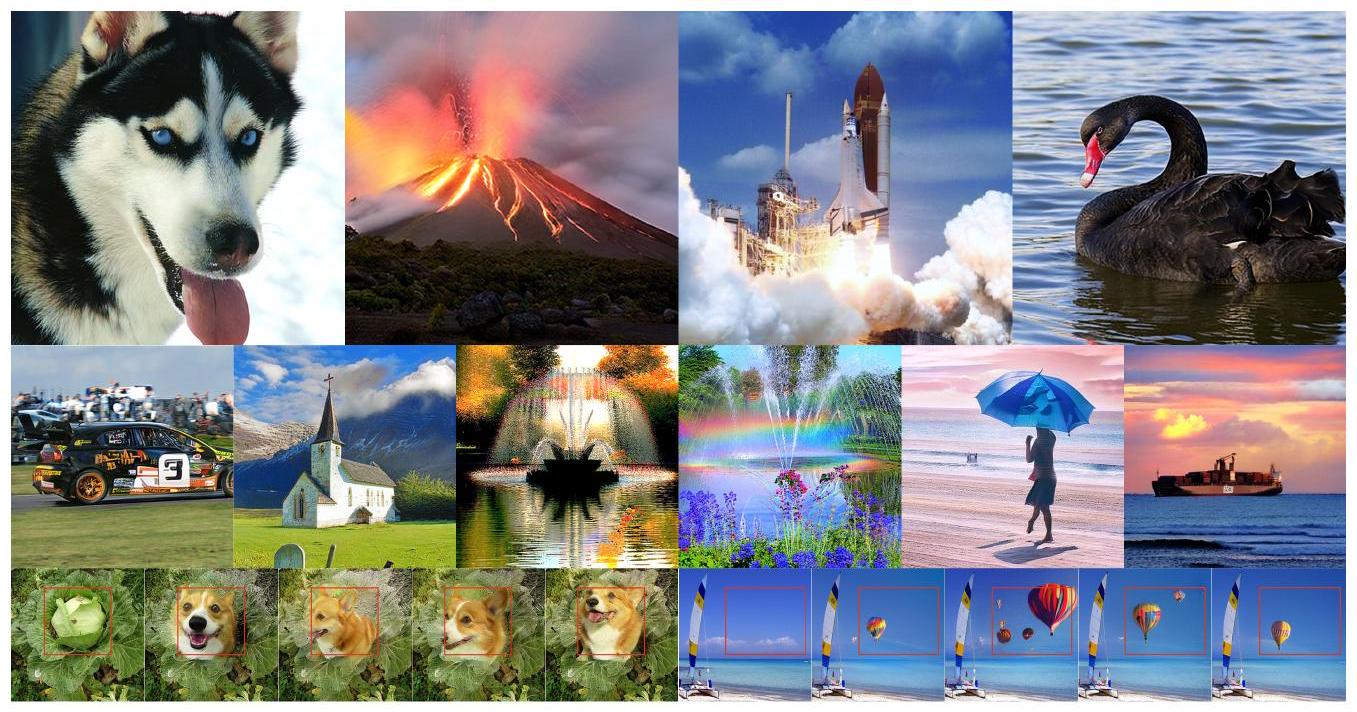
\includegraphics[width=\linewidth]{2025_10_26_62f95e615e8879e267a8g-01(1).jpg}
\caption{\textbf{Generated samples from Visual AutoRegressive (VAR) transformers trained on ImageNet.}
  We show 512$\times$512 samples (top), 256$\times$256 samples (middle), and zero-shot image editing results (bottom).}
  \label{fig:teaser}
\end{figure}

\begin{abstract}
We present Visual AutoRegressive modeling (VAR), a new generation paradigm that redefines the autoregressive learning on images as coarse-to-fine "next-scale prediction" or "next-resolution prediction", diverging from the standard raster-scan "next-token prediction". This simple, intuitive methodology allows autoregressive (AR) transformers to learn visual distributions fast and can generalize well: VAR, for the first time, makes GPT-style AR models surpass diffusion transformers in image generation. On ImageNet $256 \times 256$ benchmark, VAR significantly improve AR baseline by improving Fréchet inception distance (FID) from 18.65 to 1.73, inception score (IS) from 80.4 to 350.2 , with $20 \times$ faster inference speed. It is also empirically verified that VAR outperforms the Diffusion Transformer (DiT) in multiple dimensions including image quality, inference speed, data efficiency, and scalability. Scaling up VAR models exhibits clear power-law scaling laws similar to those observed in LLMs, with linear correlation coefficients near -0.998 as solid evidence. VAR further showcases zero-shot generalization ability in downstream tasks including image in-painting, out-painting, and editing. These results suggest VAR has initially emulated the two important properties of LLMs: Scaling Laws and zero-shot generalization. We have released all models and codes to promote the exploration of AR/VAR models for visual generation and unified learning.
\end{abstract}

\begin{figure}[h]
\begin{center}
  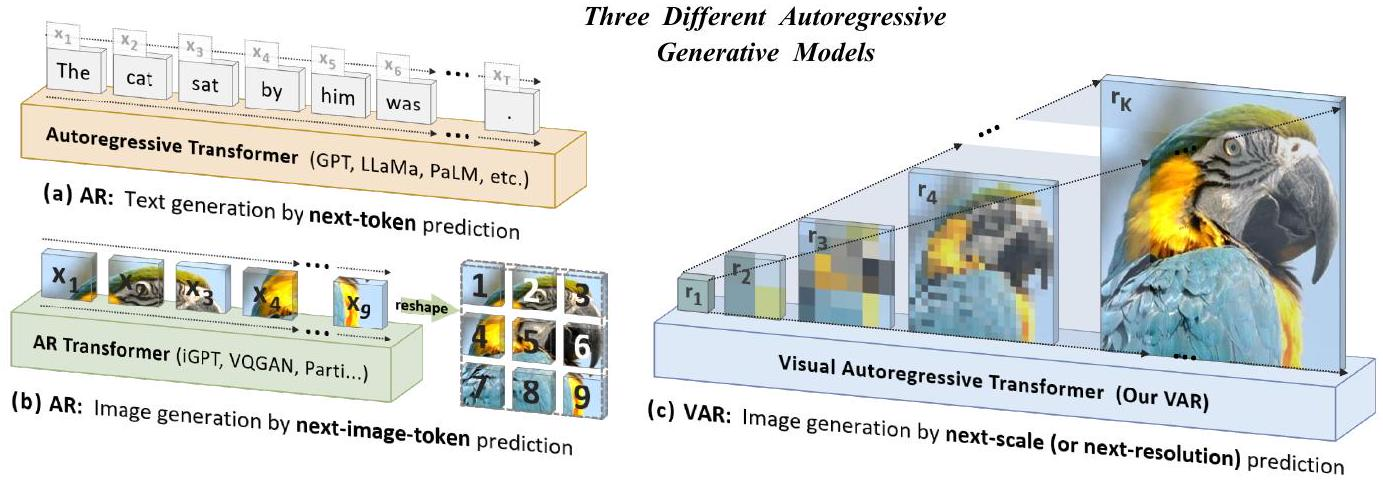
\includegraphics[width=\textwidth]{2025_10_26_62f95e615e8879e267a8g-02(1)}
\caption{Standard autoregressive modeling (AR) vs. our proposed visual autoregressive modeling (VAR). \\
(a) AR applied to language: sequential text token generation from left to right, word by word; (b) AR applied to images: sequential visual token generation in a raster-scan order, from left to right, top to bottom; (c) VAR for images: multi-scale token maps are autoregressively generated from coarse to fine scales (lower to higher resolutions), with parallel token generation within each scale. VAR requires a multi-scale VQVAE to work.}
\end{center}
\end{figure}

\section*{Introduction}
The advent of GPT series [65, 66, 15, 62, 1] and more autoregressive (AR) large language models (LLMs) [22, 4, 38, 82, 83, 90, 78, 5, 79] has heralded a new epoch in the field of artificial intelligence. These models exhibit promising intelligence in generality and versatility that, despite issues like hallucinations [39], are still considered to take a solid step toward the general artificial intelligence (AGI). At the core of these models is a self-supervised learning strategy-predicting the next token in a sequence, a simple yet profound approach. Studies into the success of these large AR models have highlighted their scalability and generalizabilty: the former, as exemplified by scaling laws [43, 35], allows us to predict large model's performance from smaller ones and thus guides better resource allocation, while the latter, as evidenced by zero-shot and few-shot learning [66, 15], underscores the unsupervised-trained models' adaptability to diverse, unseen tasks. These properties reveal AR models' potential in learning from vast unlabeled data, encapsulating the essence of "AGI".\\[0pt]
In parallel, the field of computer vision has been striving to develop large autoregressive or world models [58, 57, 6], aiming to emulate their impressive scalability and generalizability. Trailblazing efforts like VQGAN and DALL-E [30, 67] along with their successors [68, 92, 50, 99] have showcased the potential of AR models in image generation. These models utilize a visual tokenizer to discretize continuous images into grids of 2D tokens, which are then flattened to a 1D sequence for AR learning (Fig. 2b), mirroring the process of sequential language modeling (Fig. 2 a). However, the scaling laws of these models remain underexplored, and more frustratingly, their performance significantly lags behind diffusion models [63, 3, 51], as shown in Fig. 3. In contrast to the remarkable achievements of LLMs, the power of autoregressive models in computer vision appears to be somewhat locked.

Autoregressive modeling requires defining the order of data. Our work reconsiders how to "order" an image: Humans typically perceive or create images in a hierachical manner, first capturing the global structure and then local details. This multi-scale, coarse-to-fine nature suggests an "order" for images. Also inspired by the widespread multi-scale designs [54, 52, 81, 44], we define autoregressive learning for images as "next-scale prediction" in Fig. 2 (c), diverging from the conventional "next-token prediction" in Fig. 2 (b). Our approach begins by encoding an image into multi-scale token maps. The autoregressive process is then started from the $1 \times 1$ token map, and progressively expands in resolution: at each step, the transformer predicts the next higher-resolution token map conditioned on all previous ones. We refer to this methodology as Visual AutoRegressive (VAR) modeling.

\begin{figure}[h]
\begin{center}
  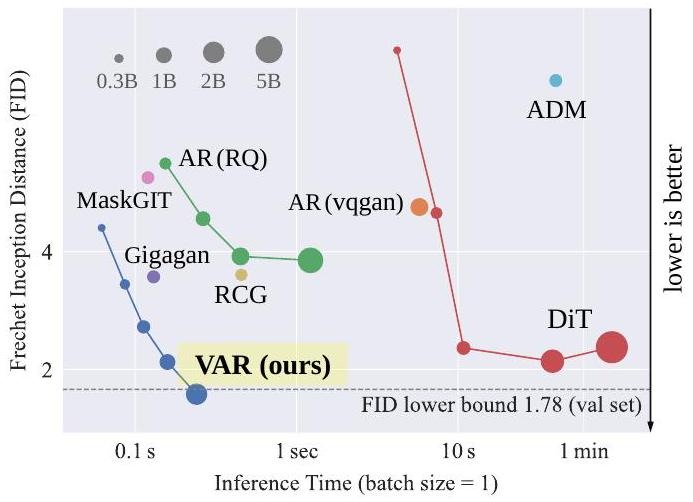
\includegraphics[width=\textwidth]{2025_10_26_62f95e615e8879e267a8g-02}
\captionsetup{labelformat=empty}
\caption{Figure 3: Scaling behavior of different model families on ImageNet $256 \times 256$ generation benchmark. The FID of the validation set serves as a reference lower bound (1.78). VAR with 2B parameters reaches an FID of 1.73 , surpassing L-DiT with 3 B or 7 B parameters.}
\end{center}
\end{figure}

VAR directly leverages GPT-2-like transformer architecture [66] for visual autoregressive learning. On the ImageNet $256 \times 256$ benchmark, VAR significantly improves its AR baseline, achieving a Fréchet inception distance (FID) of 1.73 and an inception score (IS) of 350.2 , with inference speed $20 \times$ faster (see Sec. 7 for details). Notably, VAR surpasses the Diffusion Transformer (DiT) - the foundation of leading diffusion systems like Stable Diffusion 3.0 and SORA [29, 14] - in FID/IS, data efficiency, inference speed, and scalability. VAR models also exhibit scaling laws akin to those witnessed in LLMs. Lastly, we showcase VAR's zero-shot generalization capabilities in tasks like image in-painting, out-painting, and editing. In summary, our contributions to the community include:

\begin{enumerate}
  \item A new visual generative framework using a multi-scale autoregressive paradigm with next-scale prediction, offering new insights in autoregressive algorithm design for computer vision.
  \item An empirical validation of VAR models' Scaling Laws and zero-shot generalization potential, which initially emulates the appealing properties of large language models (LLMs).
  \item A breakthrough in visual autoregressive model performance, making GPT-style autoregressive methods surpass strong diffusion models in image synthesis for the first time ${ }^{2}$.
  \item A comprehensive open-source code suite, including both VQ tokenizer and autoregressive model training pipelines, to help propel the advancement of visual autoregressive learning.
\end{enumerate}

\section*{Related Work}
\subsection*{Properties of large autoregressive language models}
Scaling laws are found and studied in autoregressive language models [43,35], which describe a power-law relationship between the scale of model (or dataset, computation, etc.) and the crossentropy loss value on the test set. Scaling laws allow us to directly predict the performance of a larger model from smaller ones [1], thus guiding better resource allocation. More pleasingly, they show that the performance of LLMs can scale well with the growth of model, data, and computation and never saturate, which is considered a key factor in the success of [15,82,83,98,90,38]. The success brought by scaling laws has inspired the vision community to explore more similar methods for multimodality understanding and generation [ $53,2,88,27,96,77,21,23,41,31,32,80,87$ ].\\[0pt]
Zero-shot generalization. Zero-shot generalization [72] refers to the ability of a model, particularly a Large Language Model, to perform tasks that it has not been explicitly trained on. Within the realm of the computer vision, there is a burgeoning interest in the zero-shot and in-context learning abilities of foundation models, CLIP [64], SAM [48], Dinov2 [61]. Innovations like Painter [89] and LVM [6] extend visual prompters [40,11] to achieve in-context learning in vision.

\subsection*{Visual generation}
Raster-scan autoregressive models for visual generation necessitate the encoding of 2D images into 1D token sequences. Early endeavors [20,84] have shown the ability to generate RGB (or grouped) pixels in the standard row-by-row, raster-scan manner. [69] extends [84] by using multiple independent trainable networks to do super-resolution repeatedly. VQGAN [30] advances [20, 84] by doing autoregressive learning in the latent space of VQVAE [85]. It employs GPT-2 decoder-only transformer to generate tokens in the raster-scan order, like how ViT [28] serializes 2D images into 1D patches. VQVAE-2 [68] and RQ-Transformer [50] also follow this raster-scan manner but use extra scales or stacked codes. Parti [93], based on the architecture of ViT-VQGAN [92], scales the transformer to 20 B parameters and works well in text-to-image synthesis.\\[0pt]
Masked-prediction model. MaskGIT [17] employs a VQ autoencoder and a masked prediction transformer similar to BERT [25, 10, 34] to generate VQ tokens through a greedy algorithm. MagViT [94] adapts this approach to videos, and MagViT-2 [95] enhances [17, 94] by introducing an improved VQVAE for both images and videos. MUSE [16] further scales MaskGIT to 3B parameters.\\[0pt]
Diffusion models' progress has centered around improved learning or sampling [76, 75, 55, 56, 7], guidance [37, 60], latent learning [70], and architectures [36, 63, 71, 91]. DiT and U-ViT [63, 8] replaces or integrates the U-Net with transformer, and inspires recent image [19, 18] or video synthesis systems [12, 33] including Stable Diffusion 3.0 [29], SORA [14], and Vidu [9].

\footnotetext{${ }^{2}$ A related work [95] named "language model beats diffusion" belongs to BERT-style masked-prediction model.
}
\section*{Method}
\subsection*{Preliminary: autoregressive modeling via next-token prediction}
Formulation. Consider a sequence of discrete tokens $x=\left(x_{1}, x_{2}, \ldots, x_{T}\right)$, where $x_{t} \in[V]$ is an integer from a vocabulary of size $V$. The next-token autoregressive posits the probability of observing the current token $x_{t}$ depends only on its prefix ( $x_{1}, x_{2}, \ldots, x_{t-1}$ ). This unidirectional token dependency assumption allows for the factorization of the sequence $x$ 's likelihood:

$$
p\left(x_{1}, x_{2}, \ldots, x_{T}\right)=\prod_{t=1}^{T} p\left(x_{t} \mid x_{1}, x_{2}, \ldots, x_{t-1}\right)
$$

Training an autoregressive model $p_{\theta}$ involves optimizing $p_{\theta}\left(x_{t} \mid x_{1}, x_{2}, \ldots, x_{t-1}\right)$ over a dataset. This is known as the "next-token prediction", and the trained $p_{\theta}$ can generate new sequences.\\[0pt]
Tokenization. Images are inherently 2D continuous signals. To apply autoregressive modeling to images via next-token prediction, we must: 1) tokenize an image into several discrete tokens, and 2) define a 1D order of tokens for unidirectional modeling. For 1), a quantized autoencoder such as [30] is often used to convert the image feature map $f \in \mathbb{R}^{h \times w \times C}$ to discrete tokens $q \in[V]^{h \times w}$ :

$$
f=\mathcal{E}(i m), \quad q=\mathcal{Q}(f)
$$

where $i m$ denotes the raw image, $\mathcal{E}(\cdot)$ a encoder, and $\mathcal{Q}(\cdot)$ a quantizer. The quantizer typically includes a learnable codebook $Z \in \mathbb{R}^{V \times C}$ containing $V$ vectors. The quantization process $q=\mathcal{Q}(f)$ will map each feature vector $f^{(i, j)}$ to the code index $q^{(i, j)}$ of its nearest code in the Euclidean sense:

$$
q^{(i, j)}=\left(\underset{v \in[V]}{\arg \min }\left\|\operatorname{lookup}(Z, v)-f^{(i, j)}\right\|_{2}\right) \in[V]
$$

where lookup $(Z, v)$ means taking the $v$-th vector in codebook $Z$. To train the quantized autoencoder, $Z$ is looked up by every $q^{(i, j)}$ to get $\hat{f}$, the approximation of original $f$. Then a new image $i \hat{m}$ is reconstructed using the decoder $\mathcal{D}(\cdot)$ given $\hat{f}$, and a compound loss $\mathcal{L}$ is minimized:

$$
\begin{aligned}
& \hat{f}=\operatorname{lookup}(Z, q), \quad i \hat{m}=\mathcal{D}(\hat{f}) \\
& \mathcal{L}=\|i m-i \hat{m}\|_{2}+\|f-\hat{f}\|_{2}+\lambda_{\mathrm{P}} \mathcal{L}_{\mathrm{P}}(i \hat{m})+\lambda_{\mathrm{G}} \mathcal{L}_{\mathrm{G}}(i \hat{m})
\end{aligned}
$$

where $\mathcal{L}_{\mathrm{P}}(\cdot)$ is a perceptual loss such as LPIPS [97], $\mathcal{L}_{\mathrm{G}}(\cdot)$ a discriminative loss like StyleGAN's discriminator loss [46], and $\lambda_{\mathrm{P}}, \lambda_{\mathrm{G}}$ are loss weights. Once the autoencoder $\{\mathcal{E}, \mathcal{Q}, \mathcal{D}\}$ is fully trained, it will be used to tokenize images for subsequent training of a unidirectional autoregressive model.

The image tokens in $q \in[V]^{h \times w}$ are arranged in a 2D grid. Unlike natural language sentences with an inherent left-to-right ordering, the order of image tokens must be explicitly defined for unidirectional autoregressive learning. Previous AR methods [30, 92, 50] flatten the 2D grid of $q$ into a 1D sequence $x=\left(x_{1}, \ldots, x_{h \times w}\right)$ using some strategy such as row-major raster scan, spiral, or z-curve order. Once flattened, they can extract a set of sequences $x$ from the dataset, and then train an autoregressive model to maximize the likelihood in (1) via next-token prediction.\\
Discussion on the weakness of vanilla autoregressive models. The above approach of tokenizing and flattening enable next-token autoregressive learning on images, but introduces several issues:

\begin{enumerate}
  \item Mathematical premise violation. In quantized autoencoders (VQVAEs), the encoder typically produces an image feature map $f$ with inter-dependent feature vectors $f^{(i, j)}$ for all $i, j$. So after quantization and flattening, the token sequence ( $x_{1}, x_{2}, \ldots, x_{h \times w}$ ) retains bidirectional correlations. This contradicts the unidirectional dependency assumption of autoregressive models, which dictates that each token $x_{t}$ should only depend on its prefix ( $x_{1}, x_{2}, \ldots, x_{t-1}$ ).
  \item Inability to perform some zero-shot generalization. Similar to issue 1), The unidirectional nature of image autoregressive modeling restricts their generalizability in tasks requiring bidirectional reasoning. E.g., it cannot predict the top part of an image given the bottom part.
  \item Structural degradation. The flattening disrupts the spatial locality inherent in image feature maps. For example, the token $q^{(i, j)}$ and its 4 immediate neighbors $q^{(i \pm 1, j)}, q^{(i, j \pm 1)}$ are closely correlated due to their proximity. This spatial relationship is compromised in the linear sequence $x$, where unidirectional constraints diminish these correlations.
  \item Inefficiency. Generating an image token sequence $x=\left(x_{1}, x_{2}, \ldots, x_{n \times n}\right)$ with a conventional self-attention transformer incurs $\mathcal{O}\left(n^{2}\right)$ autoregressive steps and $\mathcal{O}\left(n^{6}\right)$ computational cost.
\end{enumerate}

Issues 2) and 3) are evident (see examples above). Regarding issue 1), we present empirical evidence in Appendix A. The proof of issue 3) is detailed in Appendix B. These theoretical and practical limitations call for a rethinking of autoregressive models in the context of image generation.

\begin{figure}[h]
\begin{center}
  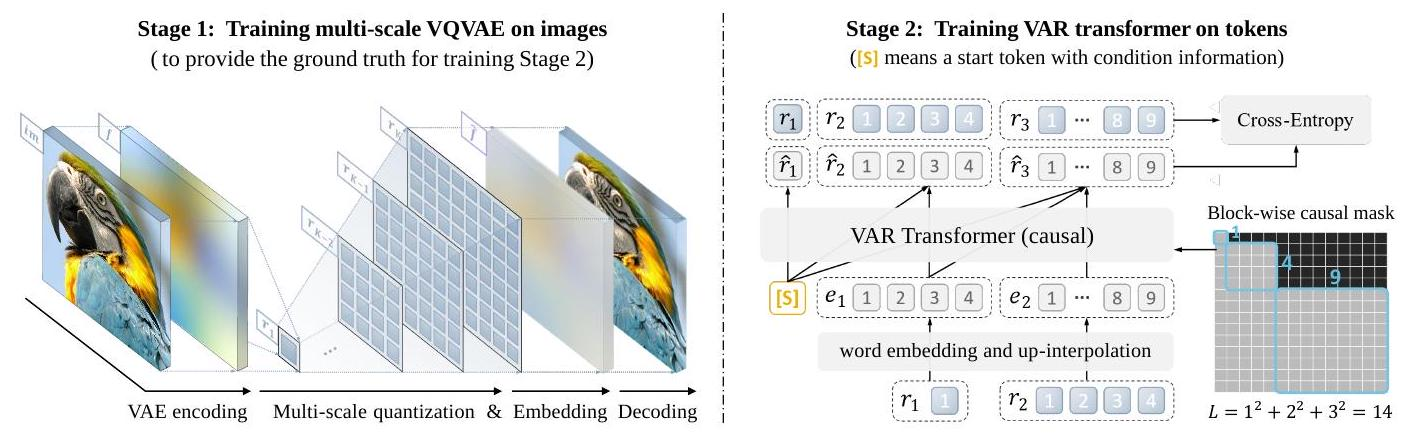
\includegraphics[width=\textwidth]{2025_10_26_62f95e615e8879e267a8g-05}
\captionsetup{labelformat=empty}
\caption{Figure 4: VAR involves two separated training stages. Stage 1: a multi-scale VQ autoencoder encodes an image into $K$ token maps \$R=\textbackslash left(r\_\{1}, r\_\{2\}, ···, r\_\{K\}\textbackslash right)\$ and is trained by a compound loss (5). For details on "Multi-scale quantization" and "Embedding", check Algorithm 1 and 2. Stage 2: a VAR transformer is trained via next-scale prediction (6): it takes ([s], $r_{1}, r_{2}, \ldots, r_{K-1}$ ) as input to predict ( $r_{1}, r_{2}, r_{3}, \ldots, r_{K}$ ). The attention mask is used in training to ensure each $r_{k}$ can only attend to $r_{\leq k}$. Standard cross-entropy loss is used.\}\end{center}
\end{figure}

\subsection*{Visual autoregressive modeling via next-scale prediction}
\textbf{Reformulation.再定式化.} We reconceptualize the autoregressive modeling on images by shifting from "nexttoken prediction" to "next-scale prediction" strategy. Here, the autoregressive unit is an entire token map, rather than a single token. We start by quantizing a feature map $f \in \mathbb{R}^{h \times w \times C}$ into $K$ multi-scale token maps ( $r_{1}, r_{2}, \ldots, r_{K}$ ), each at a increasingly higher resolution $h_{k} \times w_{k}$, culminating in $r_{K}$ matches the original feature map's resolution $h \times w$. The autoregressive likelihood is formulated as:

我々は、画像におけるオートレグレッシブモデリングを、「ネクストトークン予測」戦略から「ネクストスケール予測」戦略へと移行させることで、再概念化する [1]。ここで、オートレグレッシブの単位は、単一のトークンではなく、トークンマップ全体である [1]。我々は、特徴マップ $f \in \mathbb{R}^{h \times w \times C}$ を $K$ 個のマルチスケールトークンマップ $(r_1, r_2, \ldots, r_K)$ へと量子化することから始める [1]。これらの各マップは、次第に高くなる解像度 $h_k \times w_k$ を持ち、$r_K$ が元の特徴マップの解像度 $h \times w$ に一致する [1]。オートレグレッシブ尤度は次のように定式化される [2]:


$$
p\left(r_{1}, r_{2}, \ldots, r_{K}\right)=\prod_{k=1}^{K} p\left(r_{k} \mid r_{1}, r_{2}, \ldots, r_{k-1}\right),
$$

where each autoregressive unit $r_{k} \in[V]^{h_{k} \times w_{k}}$ is the token map at scale $k$ containing $h_{k} \times w_{k}$ tokens, and the sequence ( $r_{1}, r_{2}, \ldots, r_{k-1}$ ) serves as the the "prefix" for $r_{k}$. During the $k$-th autoregressive step, all distributions over the $h_{k} \times w_{k}$ tokens in $r_{k}$ will be generated in parallel, conditioned on $r_{k}$ 's prefix and associated $k$-th position embedding map. This "next-scale prediction" methodology is what we define as visual autoregressive modeling (VAR), depicted on the right side of Fig. 4. Note that in the training of VAR, a block-wise causal attention mask is used to ensure that each $r_{k}$ can only attend to its prefix $r_{\leq k}$. During inference, kv-caching can be used and no mask is needed.\\

ここで、各オートレグレッシブ単位 $r_k \in [V]^{h_k \times w_k}$ は、スケール $k$ における $h_k \times w_k$ 個のトークンを含むトークンマップであり、シーケンス $(r_1, r_2, \ldots, r_{k-1})$ は $r_k$ の「プレフィックス」として機能する [2]。$k$番目のオートレグレッシブステップにおいて、$r_k$ 内の $h_k \times w_k$ 個のトークンすべてにわたる分布は、$r_k$ のプレフィックスおよび関連する $k$番目の位置埋め込みマップに条件付けられ、**並列に生成される** [2]。この「ネクストスケール予測」の方法論こそが、我々が視覚オートレグレッシブモデリング(VAR)と定義するものであり、図4の右側に示されている [2]。VARの訓練では、各 $r_k$ がそのプレフィックス $r_{\le k}$ のみにアテンドできるようにするために、ブロック単位の因果的アテンションマスクが使用されることに注意されたい [2]。推論時には、kv-キャッシングを使用でき、マスクは必要ない [2]。

\textbf{Discussion.考察} VAR addresses the previously mentioned three issues as follows:
VARは、前述の3つの課題に次のように対処する [3]:


\begin{enumerate}
  \item The mathematical premise is satisfied if we constrain each $r_{k}$ to depend only on its prefix, that is, the process of getting $r_{k}$ is solely related to $r_{\leq k}$. This constraint is acceptable as it aligns with the natural, coarse-to-fine progression characteristics like human visual perception and artistic drawing (as we discussed in Sec. 1). Further details are provided in the Tokenization below.
  \item The spatial locality is preserved as (i) there is no flattening operation in VAR, and (ii) tokens in each $r_{k}$ are fully correlated. The multi-scale design additionally reinforces the spatial structure.
  \item The complexity for generating an image with $n \times n$ latent is significantly reduced to $\mathcal{O}\left(n^{4}\right)$, see Appendix for proof. This efficiency gain arises from the parallel token generation in each $r_{k}$.
\end{enumerate}

\begin{enumerate}
    \item 数学的な前提は、各 $r_k$ がそのプレフィックスにのみ依存する、すなわち、$r_k$ を取得するプロセスが $r_{\le k}$ のみに排他的に関連する場合に満たされる [3]。この制約は、人間の視覚認識や芸術的な描画に見られるような、自然な粗密(coarse-to-fine)の進行特性と一致するため、許容される(1節で議論した通り) [3]。さらなる詳細は、後述の「トークン化」で提供される [3]。
    \item 空間的な局所性は、(i)VARには平坦化操作がないこと、および(ii)各 $r_k$ 内のトークンが完全に相関していることにより、保持される [3]。マルチスケールの設計は、さらに空間構造を強化する [3]。
    \item $n \times n$ の潜在表現を持つ画像を生成するための計算量は、$O(n^4)$ に大幅に削減される(証明は付録を参照) [4]。この効率性の向上は、各 $r_k$ 内での**トークンの並列生成**から生じる [4]。
\end{enumerate}

\textbf{Tokenization.トークン化} We develope a new multi-scale quantization autoencoder to encode an image to $K$ multi-scale discrete token maps $R=\left(r_{1}, r_{2}, \ldots, r_{K}\right)$ necessary for VAR learning (6). We employ the same architecture as VQGAN [30] but with a modified multi-scale quantization layer. The encoding and decoding procedures with residual design on $f$ or $\hat{f}$ are detailed in algorithms 1 and 2. We empirically find this residual-style design, akin to [50], can perform better than independent interpolation. Algorithm 1 shows that each $r_{k}$ would depend only on its prefix ( $r_{1}, r_{2}, \ldots, r_{k-1}$ ). Note that a shared codebook $Z$ is utilized across all scales, ensuring that each $r_{k}$ 's tokens belong to\\
the same vocabulary $[V]$. To address the information loss in upscaling $z_{k}$ to $h_{K} \times w_{K}$, we use $K$ extra convolution layers $\left\{\phi_{k}\right\}_{k=1}^{K}$. No convolution is used after downsampling $f$ to $h_{k} \times w_{k}$.

我々は、VAR学習(6)に不可欠な $K$ 個のマルチスケール離散トークンマップ $R = (r_1, r_2, \ldots, r_K)$ に画像をエンコードするために、新しいマルチスケール量子化オートエンコーダを開発する [4]。我々は、VQGAN [5] と同じアーキテクチャを採用するが、マルチスケール量子化層が修正されている [4]。$f$ または $\hat{f}$ 上の残差設計を伴うエンコードおよびデコード手順は、アルゴリズム1および2に詳述されている [4]。我々は、この残差スタイルの設計が、[6]に類似しており、独立した補間よりも優れた性能を発揮することを経験的に見出した [4]。アルゴリズム1は、各 $r_k$ がそのプレフィックス $(r_1, r_2, \ldots, r_{k-1})$ にのみ依存することを示す [7]。すべてのスケールで共有コードブック $Z$ が利用され、各 $r_k$ のトークンが同じ語彙 $[V]$ に属することが保証されることに注意されたい [7]。$z_k$ を $h_K \times w_K$ にアップスケールする際の情報損失に対処するため、我々は $K$ 個の追加の畳み込み層 $\{\phi_k\}_{k=1}^K$ を使用する [7]。$f$ を $h_k \times w_k$ にダウンサンプリングした後には畳み込みは使用されない [7]。

\begin{figure}[t]
\centering
\begin{minipage}{0.47\linewidth}
\begin{algorithm}[H]
\caption{Multi-scale VQVAE Encoding}
\begin{algorithmic}[1]
\State \textbf{Inputs:} raw image $im$;
\State \textbf{Hyperparameters:} steps $K$, resolutions $(h_k, w_k)_{k=1}^{K}$;
\State $f = \mathcal{E}(im),\; R = [\;]$;
\For{$k = 1, \dots, K$}
    \State $r_k = Q(\text{interpolate}(f, h_k, w_k));$
    \State $R = \text{queue\_push}(R, r_k);$
    \State $z_k = \text{lookup}(Z, r_k);$
    \State $z_k = \text{interpolate}(z_k, h_K, w_K);$
    \State $f = f - \phi_k(z_k);$
\EndFor
\State \textbf{Return:} multi-scale tokens $R$;
\end{algorithmic}
\end{algorithm}
\end{minipage}
\hfill
\begin{minipage}{0.47\linewidth}
\begin{algorithm}[H]
\caption{Multi-scale VQVAE Reconstruction}
\begin{algorithmic}[1]
\State \textbf{Inputs:} multi-scale token maps $R$;
\State \textbf{Hyperparameters:} steps $K$, resolutions $(h_k, w_k)_{k=1}^{K}$;
\State $\hat{f} = 0$;
\For{$k = 1, \dots, K$}
    \State $r_k = \text{queue\_pop}(R);$
    \State $z_k = \text{lookup}(Z, r_k);$
    \State $z_k = \text{interpolate}(z_k, h_K, w_K);$
    \State $\hat{f} = \hat{f} + \phi_k(z_k);$
\EndFor
\State $\hat{im} = \mathcal{D}(\hat{f});$
\State \textbf{Return:} reconstructed image $\hat{im}$;
\end{algorithmic}
\end{algorithm}
\end{minipage}
\end{figure}

\section*{Implementation details 実装の詳細}

\textbf{VAR tokenizer.VARトカナイザ}
As aforementioned, we use the vanilla VQVAE architecture [30] and a multiscale quantization scheme with $K$ extra convolutions ( 0.03 M extra parameters). We use a shared codebook for all scales with $V=4096$. Following the baseline [30], our tokenizer is also trained on OpenImages [49] with the compound loss (5) and a spatial downsample ratio of $16 \times$.
前述の通り、我々は標準的なVQVAEアーキテクチャ~\cite{30}と、K個の追加の畳み込み層(0.03Mの追加パラメータ)を備えたマルチスケール量子化スキームを使用します~\cite{26, 27}。すべてのスケールに対して$V=4096$の\textbf{共有コードブック}を使用しています~\cite{26}。ベースライン~\cite{30}に従い、我々のトカナイザもOpenImages~\cite{49}で複合損失(5)を用いて訓練され、空間ダウンサンプリング比は$16\times$です~\cite{26}。

\textbf{VAR transformer.VARトランスフォーマー} Our main focus is on VAR algorithm so we keep a simple model architecture design. We adopt the architecture of standard decoder-only transformers akin to GPT-2 and VQGAN [66, 30] with adaptive normalization (AdaLN), which has widespread adoption and proven effectiveness in many visual generative models [46, 47, 45, 74, 73, 42, 63, 19]. For class-conditional synthesis, we use the class embedding as the start token [s] and also the condition of AdaLN. We found normalizing queries and keys to unit vectors before attention can stablize the training. We do not use advanced techniques in large language models, such as rotary position embedding (RoPE), SwiGLU MLP, or RMS Norm [82, 83]. Our model shape follows a simple rule like [43] that the width $w$, head counts $h$, and drop rate $d r$ are linearly scaled with the depth $d$ as follows:

我々の主眼はVARアルゴリズムにあるため、モデルアーキテクチャの設計はシンプルに保ちました。我々は、GPT-2およびVQ-GAN~[66, 30]に類似した標準的なデコーダオンリー型トランスフォーマーアーキテクチャを採用し、アダプティブ正規化(AdaLN)を組み込んでいます。これは、多くのビジュアル生成モデル[46, 47, 45, 74, 73, 42, 63, 19で広く採用され、有効性が証明されているものです[27]。クラス条件付き合成の場合、クラス埋め込みをスタートトークン$[\text{s}]$として使用し、AdaLNの条件としても使用します。アテンションの前にクエリとキーを単位ベクトルに正規化することが、訓練の安定化に役立つことを見出しました。我々は、RoPE (Rotary Position Embedding)、SwiGLU MLP、RMS Normといった大規模言語モデルで用いられる高度な技術は使用していません[82, 83]。
我々のモデル形状は、幅$w$、ヘッド数$h$、ドロップ率$dr$が深さ$d$に対して線形にスケーリングされるという、[43]のようなシンプルなルールに従っています


$$
w=64 d, \quad h=d, \quad d r=0.1 \cdot d / 24
$$

Consequently, the main parameter count $N$ of a VAR transformer with depth $d$ is given by ${ }^{3}$ :

その結果、深さ$d$を持つVARトランスフォーマーの主要なパラメータ数$N$は以下で与えられます

$$
N(d)=\underbrace{d \cdot 4 w^{2}}_{\text {self-attention }}+\underbrace{d \cdot 8 w^{2}}_{\text {feed-forward }}+\underbrace{d \cdot 6 w^{2}}_{\text {adaptive layernorm }}=18 d w^{2}=73728 d^{3} .
$$

All models are trained with the similar settings: a base learning rate of $10^{-4}$ per 256 batch size, an AdamW optimizer with $\beta_{1}=0.9, \beta_{2}=0.95$, decay $=0.05$, a batch size from 768 to 1024 and training epochs from 200 to 350 (depends on model size). The evaluations in Sec. 5 suggest that such a simple model design are capable of scaling and generalizing well.
すべてのモデルは類似の設定で訓練されました。ベース学習率はバッチサイズ256あたり$10^{-4}$、オプティマイザはAdamW($\beta_1 = 0.9, \beta_2 = 0.95$, 減衰$0.05$)、バッチサイズは768から1024、訓練エポック数は200から350です(モデルサイズに依存)。セクション5の評価は、このようなシンプルなモデル設計でも、スケーリングと汎化が十分に可能であることを示唆しています。


\section*{Empirical Results 実証結果}
This section first compares VAR with other image generative model families in Sec. 5.1. Evaluations on the scalability and generalizability of VAR models are presented in Sec. 5.2 and Appendix 6. For implementation details and ablation study, please see Appendix 4 and Appendix 7.
本セクションでは、まずセクション5.1においてVARを他の画像生成モデルファミリーと比較します。VARモデルのスケーラビリティと汎化能力に関する評価は、セクション5.2および付録6に示します。実装の詳細とアブレーション研究については、付録4および付録7をご覧ください。

\subsection*{State-of-the-art image generation 最先端の画像生成}
\textbf{Setup.セットアップ} We test VAR models with depths 16, 20, 24, and 30 on ImageNet $256 \times 256$ and $512 \times 512$ conditional generation benchmarks and compare them with the state-of-the-art image generation model families. Among all VQVAE-based AR or VAR models, VQGAN [30] and ours use the same architecture (CNN) and training data (OpenImages [49]) for VQVAE, while ViT-VQGAN [92] uses a ViT autoencoder, and both it and RQTransformer [50] trains the VQVAE directly on ImageNet. The results are summaried in Tab. 1 and Tab. 2.

我々は、深さ16、20、24、30のVARモデルをImageNet $256 \times 256$ および $512 \times 512$ の条件付き生成ベンチマークでテストし、最先端の画像生成モデルファミリーと比較します。全てのVQVAEベースのARモデルまたはVARモデルのうち、VQGAN [30] と我々のモデルは、VQVAEに**同じアーキテクチャ(CNN)と訓練データ(OpenImages [49])**を使用していますが、ViT-VQGAN [92] はViTオートエンコーダを使用しており、ViT-VQGANとRQTransformer [50] の両方がVQVAEをImageNet上で直接訓練しています。結果は表1と表2にまとめられています。

\footnotetext{${ }^{3}$ Due to resource limitation, we use a single shared adaptive layernorm (AdaLN) acorss all attention blocks in $512 \times 512$ synthesis. In this case, the parameter count would be reduced to around $12 d w^{2}+6 w^{2} \approx 49152 d^{3}$.
\\
${ }^{3}$ リソースの制約上、 $512 \times 512$ の合成において、全てのアテンションブロックで単一の共有適応型LayerNorm (AdaLN) を使用しています。この場合、パラメータ数は約 $12 d w^{2}+6 w^{2} \approx 49152 d^{3}$ に削減されます。}

\begin{table}[h]
\begin{center}
\captionsetup{labelformat=empty}
\caption{
\textbf{Generative model family comparison on class-conditional ImageNet $256\times256$
\\
クラス条件付きImageNet $256 \times 256$ における生成モデルファミリーの比較。
}
" $\downarrow$ " or " $\uparrow$ " indicate lower or higher values are better. Metrics include Fréchet inception distance (FID), inception score (IS), precision (Pre) and recall (rec). "\#Step": the number of model runs needed to generate an image. Wall-clock inference time relative to VAR is reported. Models with the suffix "-re" used rejection sampling. $\dagger$ : taken from MaskGIT [17].
\\
「$\downarrow$」または「$\uparrow$」は、値が低いほどまたは高いほど優れていることを示します。評価指標には、Fréchet Inception Distance (FID)、Inception Score (IS)、Precision (Pre)、および Recall (Rec) が含まれます。「\#Step」は、画像を生成するために必要なモデル実行の回数です。ウォールクロック推論時間はVARを基準とした相対値で報告されています。サフィックス「-re」が付いたモデルはリジェクションサンプリングを使用しました。$\dagger$:MaskGIT [17]からの引用。
}
\begin{tabular}{|l|l|l|l|l|l|l|l|l|}
\hline
Type & Model & FID $\downarrow$ & IS $\uparrow$ & Pre $\uparrow$ & Rec $\uparrow$ & \#Para & \#Step & Time \\
\hline
GAN & BigGAN [13] & 6.95 & 224.5 & 0.89 & 0.38 & 112 M & 1 & - \\
\hline
GAN & GigaGAN [42] & 3.45 & 225.5 & 0.84 & 0.61 & 569 M & 1 & - \\
\hline
GAN & StyleGan-XL [74] & 2.30 & 265.1 & 0.78 & 0.53 & 166M & 1 & 0.3 [74] \\
\hline
Diff. & ADM [26] & 10.94 & 101.0 & 0.69 & 0.63 & 554 M & 250 & 168 [74] \\
\hline
Diff. & CDM [36] & 4.88 & 158.7 & - & - & - & 8100 & - \\
\hline
Diff. & LDM-4-G [70] & 3.60 & 247.7 & - & - & 400 M & 250 & - \\
\hline
Diff. & DiT-L/2 [63] & 5.02 & 167.2 & 0.75 & 0.57 & 458M & 250 & 31 \\
\hline
Diff. & DiT-XL/2 [63] & 2.27 & 278.2 & 0.83 & 0.57 & 675M & 250 & 45 \\
\hline
Diff. & L-DiT-3B [3] & 2.10 & 304.4 & 0.82 & 0.60 & 3.0 B & 250 & >45 \\
\hline
Diff. & L-DiT-7B [3] & 2.28 & 316.2 & 0.83 & 0.58 & 7.0 B & 250 & >45 \\
\hline
Mask. & MaskGIT [17] & 6.18 & 182.1 & 0.80 & 0.51 & 227 M & 8 & 0.5 [17] \\
\hline
Mask. & RCG (cond.) [51] & 3.49 & 215.5 & - & - & 502M & 20 & 1.9 [51] \\
\hline
AR & VQVAE-2 ${ }^{\dagger}$ [68] & 31.11 & $\sim 45$ & 0.36 & 0.57 & 13.5 B & 5120 & - \\
\hline
AR & VQGAN ${ }^{\dagger}$ [30] & 18.65 & 80.4 & 0.78 & 0.26 & 227 M & 256 & 19 [17] \\
\hline
AR & VQGAN [30] & 15.78 & 74.3 & - & - & 1.4 B & 256 & 24 \\
\hline
AR & VQGAN-re [30] & 5.20 & 280.3 & - & - & 1.4 B & 256 & 24 \\
\hline
AR & ViTVQ [92] & 4.17 & 175.1 & - & - & 1.7 B & 1024 & >24 \\
\hline
AR & ViTVQ-re [92] & 3.04 & 227.4 & - & - & 1.7 B & 1024 & >24 \\
\hline
AR & RQTran. [50] & 7.55 & 134.0 & - & - & 3.8 B & 68 & 21 \\
\hline
AR & RQTran.-re [50] & 3.80 & 323.7 & - & - & 3.8 B & 68 & 21 \\
\hline
VAR & VAR-d16 & 3.30 & 274.4 & 0.84 & 0.51 & 310 M & 10 & 0.4 \\
\hline
VAR & VAR-d20 & 2.57 & 302.6 & 0.83 & 0.56 & 600M & 10 & 0.5 \\
\hline
VAR & VAR-d24 & 2.09 & 312.9 & 0.82 & 0.59 & 1.0 B & 10 & 0.6 \\
\hline
VAR & VAR-d30 & 1.92 & 323.1 & 0.82 & 0.59 & 2.0 B & 10 & 1 \\
\hline
VAR & VAR-d30-re & 1.73 & 350.2 & 0.82 & 0.60 & 2.0 B & 10 & 1 \\
\hline
 & (validation data) & 1.78 & 236.9 & 0.75 & 0.67 &  &  &  \\
\hline
\end{tabular}
\end{center}
\end{table}

\textbf{Overall comparison.全体比較。} In comparison with existing generative approaches including generative adversarial networks (GAN), diffusion models (Diff.), BERT-style masked-prediction models (Mask.), and GPT-style autoregressive models (AR), our visual autoregressive (VAR) establishes a new model class. As shown in Tab. 1, VAR not only achieves the best FID/IS but also demonstrates remarkable speed in image generation. VAR also maintains decent precision and recall, confirming its semantic consistency. These advantages hold true on the $512 \times 512$ synthesis benchmark, as detailed in Tab. 2 . Notably, VAR significantly advances traditional AR capabilities. To our knowledge, this is the first time of autoregressive models outperforming Diffusion transformers, a milestone made possible by VAR's resolution of AR limitations discussed in Section 3.

既存の生成手法、すなわち敵対的生成ネットワーク(GAN)、拡散モデル(Diff.)、BERTスタイルのマスク予測モデル(Mask.)、およびGPTスタイルの自己回帰モデル(AR)と比較して、我々のVisual Auto-Regressive(VAR)は、新しいモデルクラスを確立します。表1に示すように、VARは最高のFID/ISを達成するだけでなく、画像生成において驚異的な速度も示しています。VARはまた、適切なPrecisionとRecallを維持しており、そのセマンティックな一貫性を裏付けています。これらの優位性は、表2に詳述されているように、$512 \times 512$ の合成ベンチマークでも当てはまります。特筆すべきは、VARが従来のARの能力を大きく前進させた点です。我々の知る限り、自己回帰モデルが拡散トランスフォーマーを凌駕したのはこれが初めてであり、これはセクション3で議論されたARの限界をVARが解消したことによって可能になった画期的な成果です。

\textbf{Efficiency comparison.効率性の比較} Conventional autoregressive (AR) models [30, 68, 92, 50] suffer a lot from the high computational cost, as the number of image tokens is quadratic to the image resolution. A full autoregressive generation of $n^{2}$ tokens requires $\mathcal{O}\left(n^{2}\right)$ decoding iterations and $\mathcal{O}\left(n^{6}\right)$ total computations. In contrast, VAR only requires $\mathcal{O}(\log (n))$ iterations and $\mathcal{O}\left(n^{4}\right)$ total computations. The wall-clock time reported in Tab. 1 also provides empirical evidence that VAR is around 20 times faster than VQGAN and ViT-VQGAN even with more model parameters, reaching the speed of efficient GAN models which only require 1 step to generate an image.

従来の自己回帰(AR)モデル [30, 68, 92, 50] は、画像トークンの数が画像解像度の2乗に比例するため、高い計算コストに大きく悩まされます。$n^2$ 個のトークンを完全に自己回帰生成するには、$\mathcal{O}(n^2)$ のデコード反復と $\mathcal{O}(n^6)$ の総計算コストが必要です。対照的に、VARは $\mathcal{O}(\log(n))$ の反復と $\mathcal{O}(n^4)$ の総計算コストしか必要としません。表1で報告されている実測時間(ウォールクロックタイム)もまた、VARがより多くのモデルパラメータを持っているにもかかわらず、VQGANやViT-VQGANよりも約20倍高速であり、画像を生成するのに1ステップしか必要としない効率的なGANモデルの速度に達しているという経験的証拠を提供しています。

\begin{table}[h]
\begin{center}
\caption{\textbf{ImageNet $512\times512$ conditional generation.} $\dagger$ : quoted from MaskGIT [17]. "-s": a single shared AdaLN layer is used due to resource limitation.
\textbf{ImageNet $512\times512$ 条件付き生成} $\dagger$:MaskGIT [17] から引用。 「-s」:リソースの制約により、単一の共有 AdaLN(Adaptive Layer Normalization)層を使用。
}
\begin{tabular}{c|l|ccc}
\hline
Type & Model & FID $\downarrow$ & IS $\uparrow$ & Time \\
\hline
GAN & BigGAN [13] & 8.43 & 177.9 & - \\
\hline
Diff. & ADM [26] & 23.24 & 101.0 & - \\
Diff. & DiT-XL/2 [63] & 3.04 & 240.8 & 81 \\
\hline
Mask. & MaskGIT [17] & 7.32 & 156.0 & $0.5^{\dagger}$ \\
\hline
AR & VQGAN [30] & 26.52 & 66.8 & $25^{\dagger}$ \\
VAR & VAR- $d 36-\mathrm{s}$ & $\mathbf{2 . 6 3}$ & $\mathbf{3 0 3 . 2}$ & 1 \\
\hline
\end{tabular}
\end{center}
\end{table}

\textbf{Compared with popular diffusion transformer.} The VAR model surpasses the recently popular diffusion models iffusion Transformer (DiT), which serves as the precursor to the latest StableDiffusion 3 [29] and SORA [14], in multiple dimensions: 
我々のVARモデルは、最新のStable Diffusion 3 [29] やSORA [14] の先駆けとなる、最近人気の高い拡散モデルであるDiffusion Transformer (DiT) を、多岐にわたる側面で上回っています。

1) In image generation diversity and quality(FID and IS), VAR with 2B parameters consistently performs better than DiT-XL/2 [63], L-DiT-3B, and L-DiT-7B [3]. VAR also maintains comparable precision and recall.
画像生成の多様性と品質(FIDおよびIS) において、20億パラメータを持つVARは、DiT-XL/2 [63]、L-DiT-3B、およびL-DiT-7B [3] よりも一貫して優れた性能を発揮します。また、VARは同等の Precision(適合率)と Recall(再現率)を維持しています。

2) For inference speed, the DiT-XL/2 requires $45 \times$ the wall-clock time compared to VAR, while 3 B and 7B models [3] would cost much more. 
推論速度に関して、 DiT-XL/2 はVARと比較して45倍の実測時間(ウォールクロックタイム)を要し、30億および70億パラメータのモデル [3] はさらに多くのコストがかかります。

3) VAR is considered more data-efficient, as it requires only 350 training epochs compared to DiT-XL/2's 1400. 
VARはよりデータ効率が高いと見なされます。これは、DiT-XL/2の1400訓練エポックに対し、VARはわずか350エポックしか必要としないためです。

4) For scalability, Fig. 3 and Tab. 1 show that DiT only obtains marginal or even negative gains beyond 675 M parameters. In contrast, the FID and IS of VAR are consistently improved, aligning with the scaling law study in Sec. 5.2. These results establish VAR as potentially a more efficient and scalable model for image generation than models like DiT.
スケーラビリティに関して、 図3および表1に示すように、DiTは6億7500万パラメータを超えると、わずかな改善しか得られないか、負のゲインすら示します。対照的に、VARのFIDとISは一貫して改善しており、セクション5.2のスケーリング則の研究と整合しています。

\begin{figure}[h]
\begin{center}
  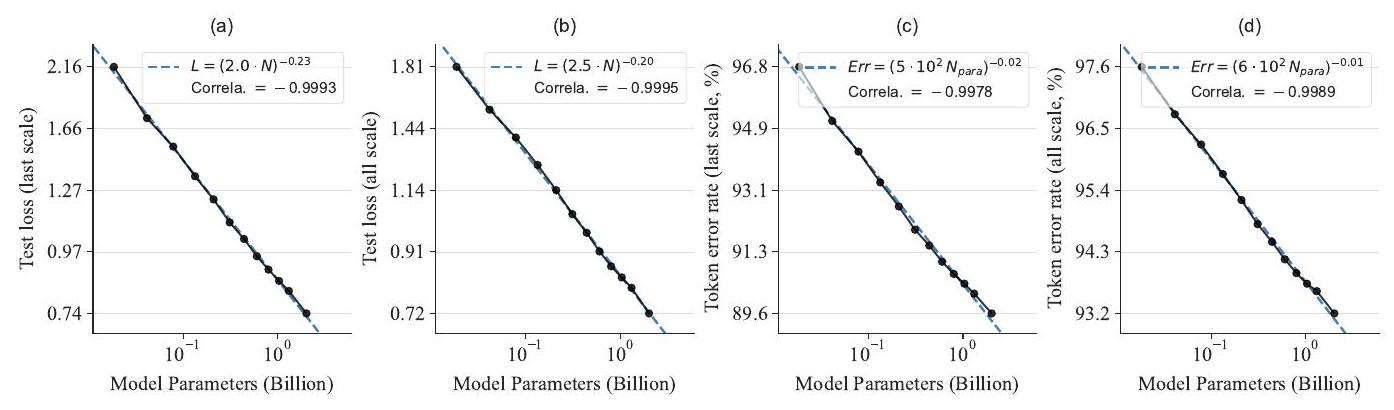
\includegraphics[width=\textwidth]{2025_10_26_62f95e615e8879e267a8g-08}
\caption{\textbf{Scaling laws with VAR transformer size $N$,}with power-law fits (dashed) and equations (in legend). Small, near-zero exponents $\alpha$ suggest a smooth decline in both test loss $L$ and token error rate $E r r$ when scaling up VAR transformer. Axes are all on a logarithmic scale. The Pearson correlation coefficients near -0.998 signify a strong linear relationship between $\log (N)$ vs. $\log (L)$ or $\log (N)$ vs. $\log (E r r)$.}
\textbf{VARトランスフォーマーのサイズ $N$ に関するスケーリング則}べき乗則によるフィッティング(破線)と(凡例中の)数式を示しています。小さい、ゼロに近い指数 $\alpha$ は、VARトランスフォーマーをスケールアップする際に、テスト損失 $L$ とトークンエラー率 $Err$ の両方が滑らかに減少することを示唆しています。軸はすべて対数スケールです。ピアソン相関係数が$-0.998$に近いことは、$\log(N)$ と $\log(L)$ または $\log(N)$ と $\log(Err)$ の間に強い線形関係があることを示しています。
\end{center}
\end{figure}

\subsection{Power-law scaling laws べき乗則によるスケーリング則}
\textbf{Background.背景} Prior research [43, 35, 38, 1] have established that scaling up autoregressive (AR) large language models (LLMs) leads to a predictable decrease in test loss $L$. This trend correlates with parameter counts $N$, training tokens $T$, and optimal training compute $C_{\min }$, following a power-law:

従来の研究 [43, 35, 38, 1] により、自己回帰型(AR)大規模言語モデル(LLMs)をスケールアップすると、テスト損失 $L$ が予測可能な形で減少することが確立されています。この傾向は、パラメータ数 $N$、訓練トークン数 $T$、および最適訓練計算量 $C_{\min}$ と相関しており、以下の**べき乗則**に従います。

$$
L=(\beta \cdot X)^{\alpha},
$$

where $X$ can be any of $N, T$, or $C_{\min }$. The exponent $\alpha$ reflects the smoothness of power-law, and $L$ denotes the reducible loss normalized by irreducible loss $L_{\infty}[35]^{4}$. A logarithmic transformation to $L$ and $X$ will reveal a linear relation between $\log (L)$ and $\log (X)$ :

ここで、$X$ は $N, T,$ または $C_{\min}$ のいずれかであり、指数 $\alpha$ はべき乗則の滑らかさを反映し、$L$ は既約損失 $L_{\infty}$ [35]$^{4}$ によって正規化された**可約損失**を示します。 $L$ と $X$ に対して対数変換を行うと、$\log(L)$ と $\log(X)$ の間に線形関係が現れます。

$$
\log (L)=\alpha \log (X)+\alpha \log \beta .
$$

An appealing phenomenon is that both [43] and [35] never observed deviation from these linear relationships at the higher end of $X$, although flattening is inevitable as the loss approaches zero.

魅力的な現象として、損失がゼロに近づくにつれて平坦化は避けられないものの、[43]と[35]のどちらにおいても、$X$ の高い側でこれらの線形関係からの逸脱は観察されませんでした。

These observed scaling laws [43, 35, 38, 1] not only validate the scalability of LLMs but also serve as a predictive tool for AR modeling, which facilitates the estimation of performance for larger AR models based on their smaller counterparts, thereby saving resource usage by large model performance forecasting. Given these appealing properties of scaling laws brought by LLMs, their replication in computer vision is therefore of significant interest.

これらの観測されたスケーリング則 [43, 35, 38, 1] は、LLMのスケーラビリティを裏付けるだけでなく、ARモデリングのための**予測ツール**としても機能します。これにより、より小さなARモデルに基づいてより大きなARモデルの性能を推定することが容易になり、大規模モデルの性能予測にかかるリソース使用量を節約できます。LLMによってもたらされるスケーリング則のこれらの魅力的な特性を鑑みると、コンピュータービジョン分野でのそれらの再現は、したがって非常に重要です。

\textbf{Setup of scaling VAR models.VARモデルのスケーリング設定} Following the protocols from [43, 35, 38, 1], we examine whether our VAR model complies with similar scaling laws. We trained models across 12 different sizes, from 18M to 2B parameters, on the ImageNet training set [24] containing 1.28M images (or 870B image tokens under our VQVAE) per epoch. For models of different sizes, training spanned 200 to 350 epochs, with a maximum number of tokens reaching 305 billion. Below we focus on the scaling laws with model parameters $N$ and optimal training compute $C_{\min }$ given sufficient token count $T$.

[43, 35, 38, 1] のプロトコルに従い、我々のVARモデルが同様のスケーリング則に準拠するかどうかを検証します。我々は、18Mから2Bパラメータまでの12種類の異なるサイズを持つモデルを、ImageNet訓練セット [24] で訓練しました。この訓練セットは、エポックあたり128万枚の画像(または我々のVQVAEの下では8700億枚の画像トークン)を含んでいます。異なるサイズのモデルに対して、訓練は200から350エポックに及び、最大トークン数は3050億に達しました。以下では、十分なトークンカウント $T$ が与えられた場合の、モデルパラメータ $N$ および最適訓練計算量 $C_{\min}$ に関するスケーリング則に焦点を当てます。

\textbf{Scaling laws with model parameters $N$.} We first investigate the test loss trend as the VAR model size increases. The number of parameters $N(d)=73728 d^{3}$ for a VAR transformer with depth $d$ is specified in (8). We varied $d$ from 6 to 30 , yielding 12 models with 18.5 M to 2.0 B parameters. We assessed the final test cross-entropy loss $L$ and token prediction error rates $E r r$ on the ImageNet validation set of 50,000 images [24]. We computed $L$ and $E r r$ for both the last scale (at the last next-scale autoregressive step), as well as the global average. Results are plotted in Fig. 5, where weobserved a clear power-law scaling trend for $L$ as a function of $N$, as consistent with [43,35,38,1]. The power-law scaling laws can be expressed as:

まず、VARモデルのサイズが増加するにつれてのテスト損失の傾向を調査します。深さ $d$ のVARトランスフォーマーのパラメータ数 $N(d) = 73728 d^3$ は (8) で指定されています。我々は $d$ を6から30まで変化させ、1850万から20億パラメータを持つ12個のモデルを得ました。我々は、50,000枚の画像からなるImageNet検証セット [24] において、最終的なテストクロスエントロピー損失 $L$ とトークン予測エラー率 $Err$ を評価しました。我々は $L$ と $Err$ を、最後のスケール(最後の次スケール自己回帰ステップ)と、グローバル平均の両方について計算しました。結果を図5にプロットしており、[43, 35, 38, 1] と同様に、$N$ の関数として $L$ に明確な**べき乗則のスケーリング傾向**が観察されました。このべき乗則によるスケーリング則は、以下のように表現できます。

\footnotetext{${ }^{4}$ See [35] for some theoretical explanation on scaling laws on negative-loglikelihood losses.
}

\begin{figure}[h]
\begin{center}
  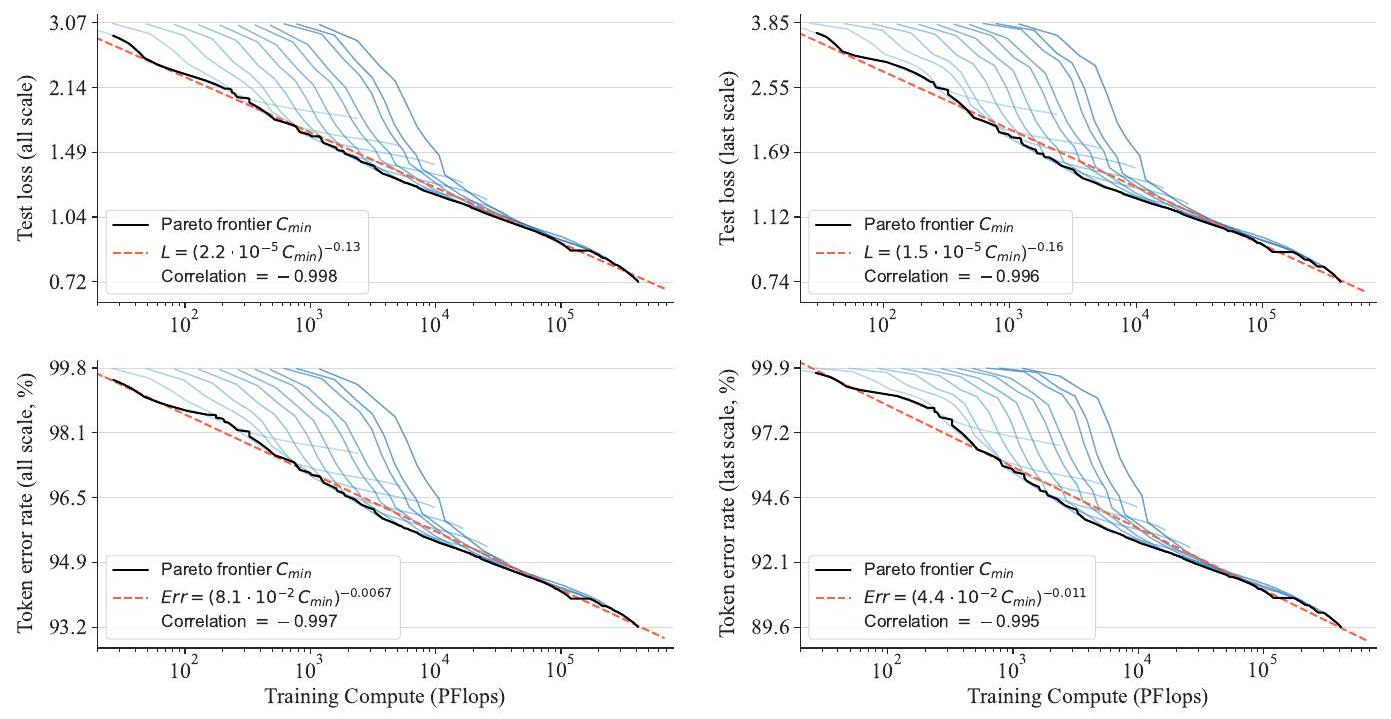
\includegraphics[width=\textwidth]{2025_10_26_62f95e615e8879e267a8g-09}
\caption{
\textbf{Scaling laws with optimal training compute$C_\mathrm{min}$
\\
最適な訓練計算量 $C_{\text{min}}$ に関するスケーリング則}.
\\
Line color denotes different model sizes. Red dashed lines are power-law fits with equations in legend. Axes are on a logarithmic scale. Pearson coefficients near -0.99 indicate strong linear relationships between $\log\left(C_\mathrm {min}\right)$ vs. $\log(L)$ or $\log \left(C_\mathrm{min}\right)$ vs. $\log(Err)$.
\\
線の色は異なるモデルサイズを示します。赤い破線は、凡例中に数式が示されている**べき乗則によるフィッティング**です。軸はすべて対数スケールで表示されています。ピアソン相関係数が$-0.99$に近いことは、$\log(C_{\text{min}})$ と $\log(L)$、または $\log(C_{\text{min}})$ と $\log(Err)$ の間に**強い線形関係**があることを示しています。
}

\end{center}
\end{figure}


$$
L_{\text {last }}=(2.0 \cdot N)^{-0.23} \quad \text { and } \quad L_{\text {avg }}=(2.5 \cdot N)^{-0.20} .
$$

Although the scaling laws are mainly studied on the test loss, we also empirically observed similar power-law trends for the token error rate $Err$:

スケーリング則は主にテスト損失で研究されていますが、我々はトークンエラー率 $Err$ についても同様のべき乗則の傾向を経験的に観察しました。

$$
E r r_{\text {last }}=\left(4.9 \cdot 10^{2} N\right)^{-0.016} \text { and } E r r_{\text {avg }}=\left(6.5 \cdot 10^{2} N\right)^{-0.010} .
$$

These results verify the strong scalability of VAR, by which scaling up VAR transformers can continuously improve the model's test performance.

これらの結果は、VARトランスフォーマーをスケールアップすることでモデルのテスト性能が継続的に向上するという、VARの強力なスケーラビリティを実証しています。

\textbf{Scaling laws with optimal training compute $C_{\min }$.最適な訓練計算量 $C_{\text{min}}$ に関するスケーリング則} We then examine the scaling behavior of VAR transformers when increasing training compute $C$. For each of the 12 models, we traced the test loss $L$ and token error rate $Err$ as a function of $C$ during training quoted in PFlops ( $10^{15}$ floating-point operations per second).
The results are plotted in Fig. 6. Here, we draw the Pareto frontier of $L$ and $E r r$ to highlight the optimal training compute $C_{\text {min }}$ required to reach a certain value of loss or error.

次に、訓練計算量 $C$ を増加させた場合のVARトランスフォーマーのスケーリング挙動を検証します。12個の各モデルについて、訓練中にテスト損失 $L$ とトークンエラー率 $\operatorname{Err}$ を、PFlops($10^{15}$ 浮動小数点演算/秒)で示される $C$ の関数として追跡しました。
結果を図6にプロットしています。ここで、損失またはエラーの特定の値に到達するために必要な最適訓練計算量 $C_{\text{min}}$ を強調するために、$L$ と $\operatorname{Err}$ のパレートフロンティアを描画します。

The fitted power-law scaling laws for $L$ and $\operatorname{Err}$ as a function of $C_{\min }$ are:

$C_{\text{min}}$ の関数としての $L$ と $\operatorname{Err}$ に対するフィッティングされたべき乗則スケーリング則は以下の通りです。

$$
\begin{aligned}
& L_{\text {last }}=\left(2.2 \cdot 10^{-5} C_{\min }\right)^{-0.13} \\
& L_{\text {avg }}=\left(1.5 \cdot 10^{-5} C_{\min }\right)^{-0.16} \\
& \operatorname{Err}_{\text {last }}=\left(8.1 \cdot 10^{-2} C_{\min }\right)^{-0.0067} \\
& \operatorname{Err}_{\text {avg }}=\left(4.4 \cdot 10^{-2} C_{\min }\right)^{-0.011}
\end{aligned}
$$

These relations $(14,16)$ hold across 6 orders of magnitude in $C_{\min }$, and our findings are consistent with those in [43, 35]: when trained with sufficient data, larger VAR transformers are more computeefficient because they can reach the same level of performance with less computation.

これらの関係式 $(14, 16)$ は $C_{\text{min}}$ の6桁にわたって成立しており、我々の知見は [43, 35] の結果と一致しています。すなわち、十分なデータで訓練された場合、より大きなVARトランスフォーマーは、同じレベルの性能をより少ない計算量で達成できるため、計算効率が高いと言えます。

\section{Visualization of scaling effect スケーリング効果の可視化}
To better understand how VAR models are learning when scaled up, we compare some generated $256 \times 256$ samples from VAR models of 4 different sizes (depth 6, 16, 26, 30) and 3 different training stages ( $20 \%, 60 \%, 100 \%$ of total training tokens) in Fig. 7. To keep the content consistent, a same random seed and teacher-forced initial tokens are used. The observed improvements in visual fidelity and soundness are consistent with the scaling laws, as larger transformers are thought able to learn more complex and fine-grained image distributions.

VARモデルがスケールアップする際にどのように学習しているかをよりよく理解するために、図7において、4つの異なるサイズ(深さ6, 16, 26, 30)と3つの異なる訓練ステージ(総訓練トークン数の20\%、60\%、100\%)のVARモデルから生成された$256 \times 256$のサンプルを比較します。内容の一貫性を保つため、同一のランダムシードとティーチャーフォースされた初期トークンを使用しています。観察された視覚的忠実度と健全性の改善は、スケーリング則と一致しています。これは、より大きなトランスフォーマーが、より複雑で詳細な画像分布を学習できると考えられるためです。

\begin{figure}[t]
\begin{center}
  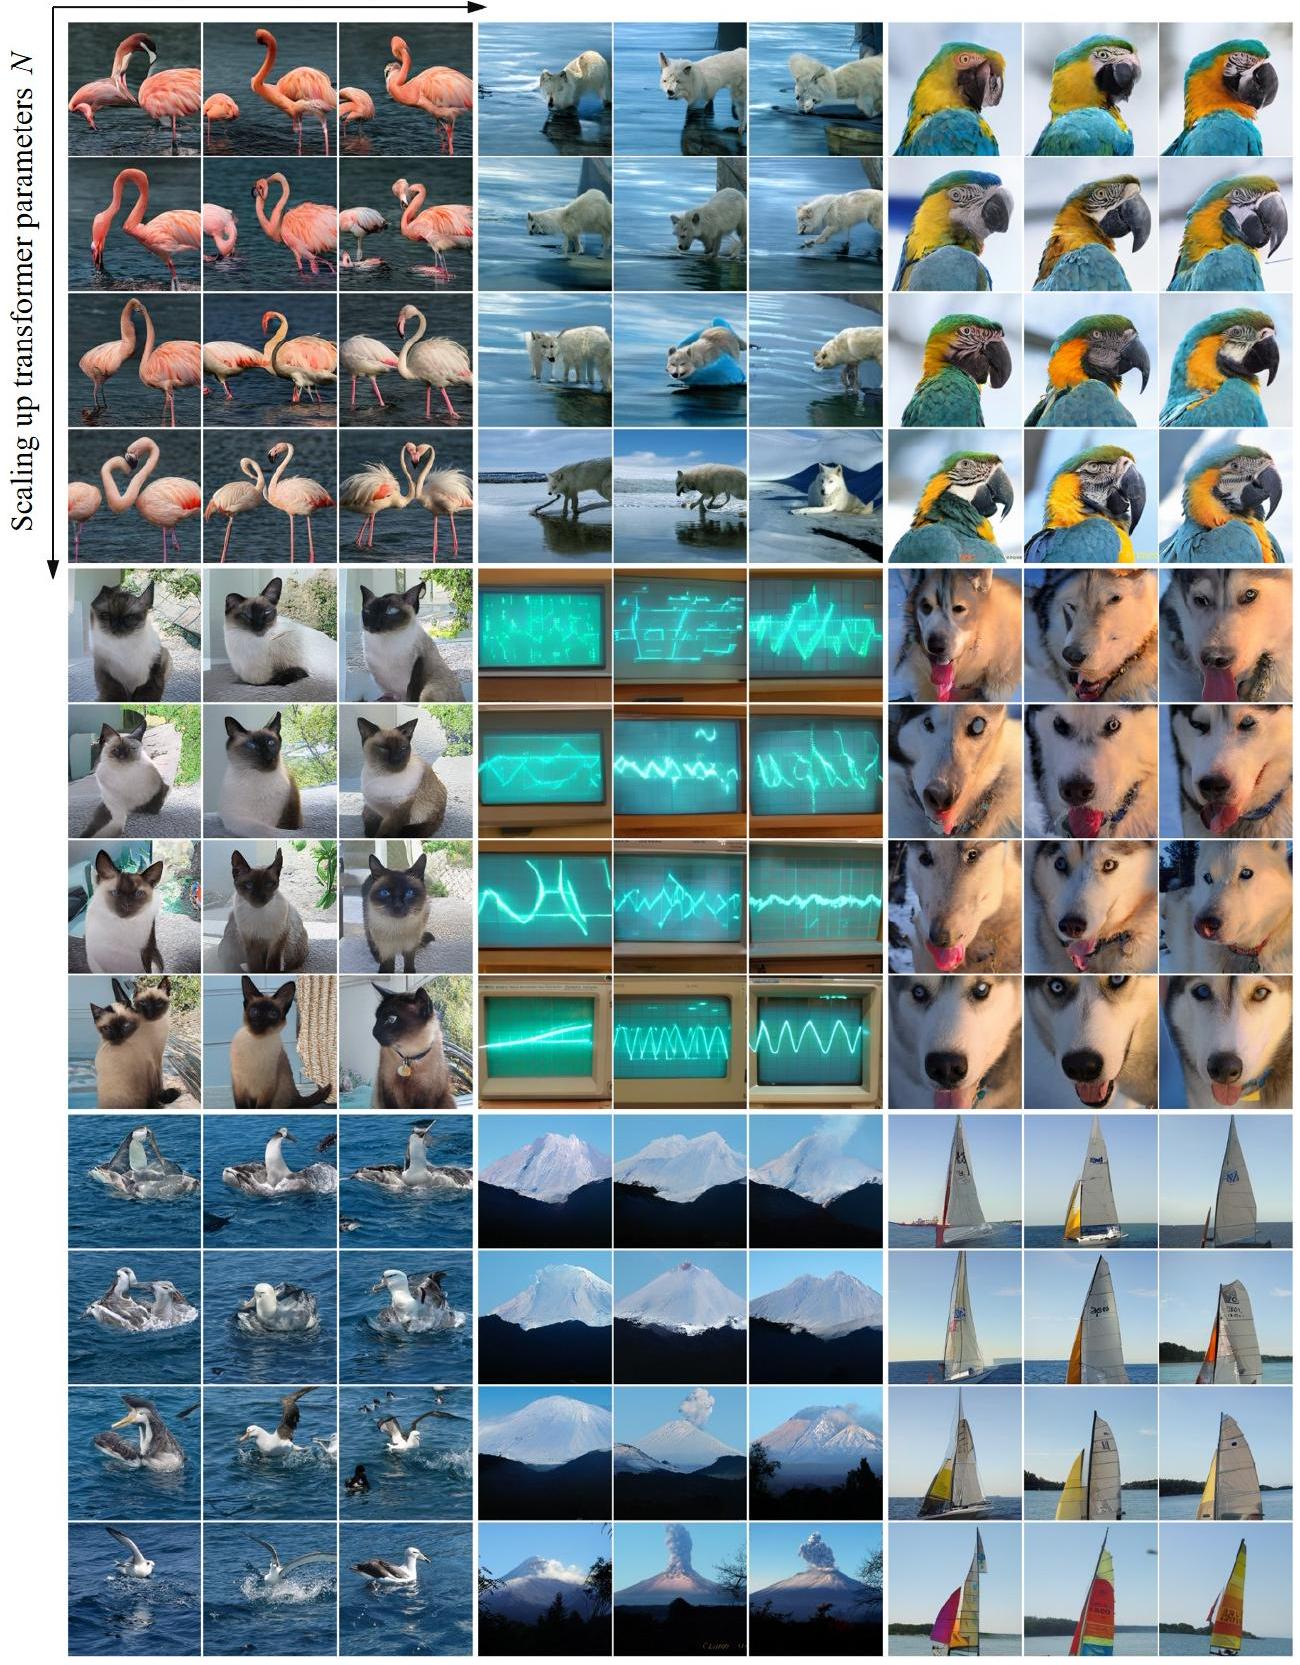
\includegraphics[width=0.8\textwidth]{2025_10_26_62f95e615e8879e267a8g-10}
\caption{\textbf{Scaling model size $N$ and training compute $C$ improves visual fidelity and soundness.}
Zoom in for a better view. Samples are drawn from VAR models of 4 different sizes and 3 different training stages. 9 class labels (from left to right, top to bottom) are: flamingo 130, arctic wolf 270, macaw 88, Siamese cat 284, oscilloscope 688 , husky 250 , mollymawk 146 , volcano 980 , and catamaran 484.
\textbf{モデルサイズ $N$ と訓練計算量 $C$ のスケーリングによる視覚的忠実度と健全性の改善。}
拡大して詳細を確認してください。サンプルは、4種類の異なるサイズのVARモデルと、3つの異なる訓練ステージから抽出されたものです。9種類のクラスラベル(左から右、上から下)は、フラミンゴ 130、ホッキョクオオカミ 270、コンゴウインコ 88、シャムネコ 284、オシロスコープ 688、ハスキー 250、モリーモーク 146、火山 980、カタマラン 484です。
}
\end{center}
\end{figure}

\section{Zero-shot task generalization ゼロショット・タスク汎化}

\textbf{Image in-painting and out-painting.} VAR- $d 30$ is tested. For in- and out-painting, we teacher-force ground truth tokens outside the mask and let the model only generate tokens within the mask. No class label information is injected into the model. The results are visualized in Fig. 8. Without modifications to the network architecture or tuning parameters, VAR has achieved decent results on these downstream tasks, substantiating the generalization ability of VAR.

\textbf{画像インペインティングおよびアウトペインティング。} VAR-d30(深さ30のVARモデル)でテストを行いました。インペインティングおよびアウトペインティングでは、マスク外のグラウンドトルーストークンをティーチャーフォースし、モデルにはマスク内のトークンのみを生成させます。クラスラベル情報はモデルに注入していません。結果を図8に可視化しています。ネットワークアーキテクチャの変更やパラメータのチューニングを行うことなく、VARはこれらのダウンストリームタスクで適切な結果を達成しており、VARの汎化能力を実証しています。

\textbf{Class-conditional image editing.} Following MaskGIT [17] we also tested VAR on the classconditional image editing task. Similar to the case of in-painting, the model is forced to generate tokens only in the bounding box conditional on some class label. Fig. 8 shows the model can produce plausible content that fuses well into the surrounding contexts, again verifying the generality of VAR.

\textbf{クラス条件付き画像編集。} MaskGIT [17] に倣い、我々はVARをクラス条件付き画像編集タスクでもテストしました。インペインティングの場合と同様に、モデルは特定のクラスラベルを条件としてバウンディングボックス内のトークンのみを生成するように強制されます。図8は、モデルが周囲の文脈にうまく融合するもっともらしい内容を生成できることを示しており、VARの汎用性を再び検証しています。

\begin{figure}[h]
\begin{center}
  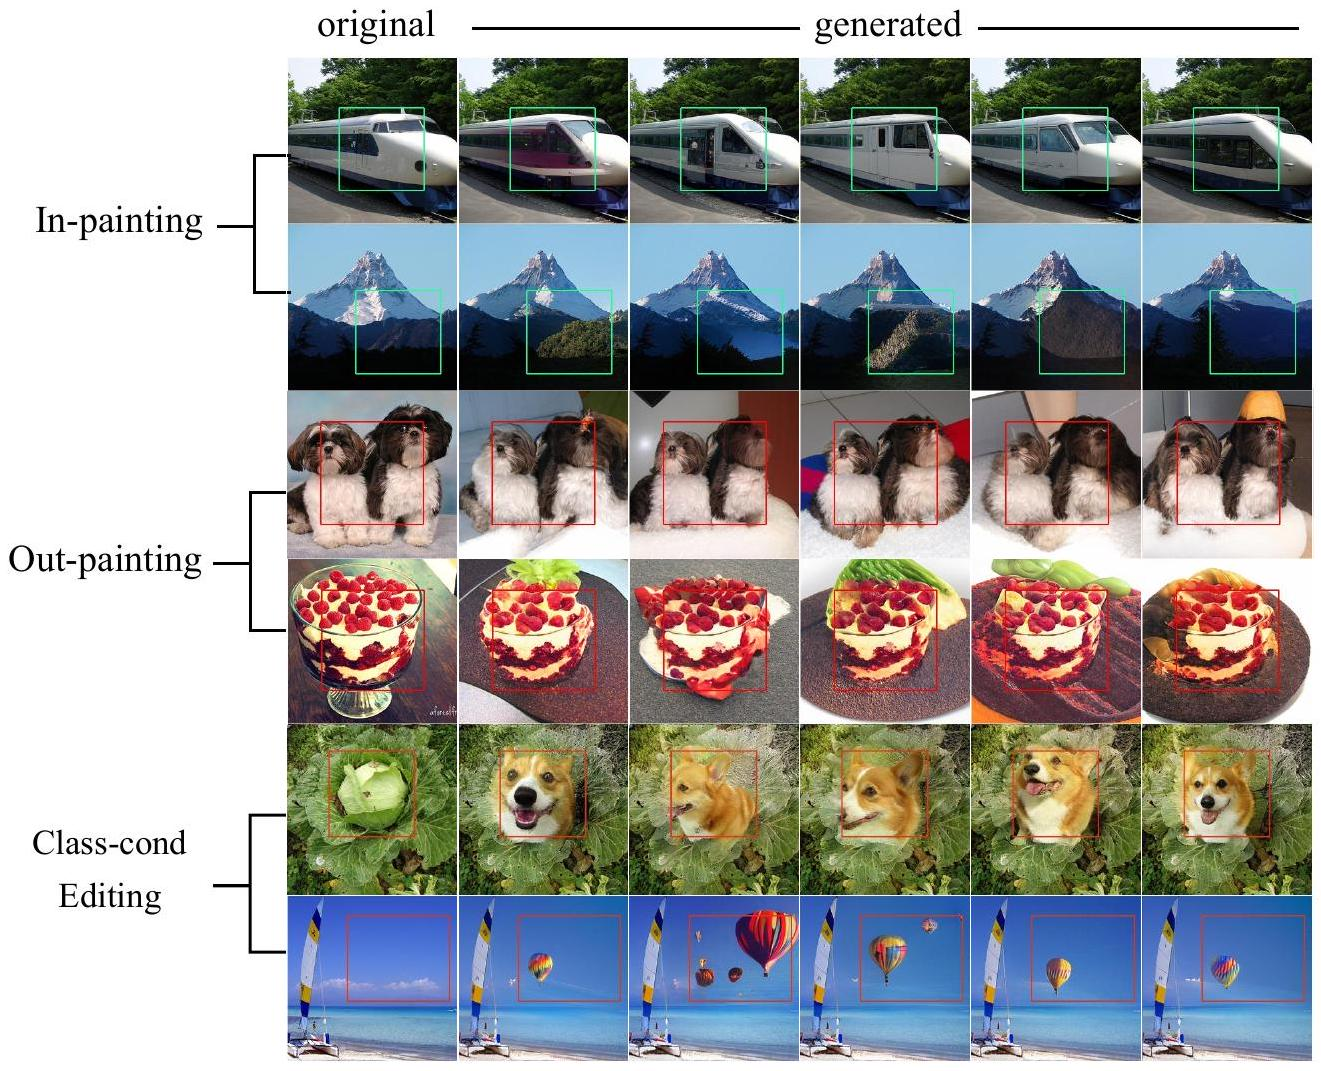
\includegraphics[width=\textwidth]{2025_10_26_62f95e615e8879e267a8g-11}
\caption{\textbf{Zero-shot evaluation in downstream tasks} containing in-painting, out-painting, and classconditional editing. The results show that VAR can generalize to novel downstream tasks without special design and finetuning. Zoom in for a better view.
\textbf{ダウンストリームタスクにおけるゼロショット評価}(インペインティング、アウトペインティング、クラス条件付き編集を含む)。結果は、VARが特別な設計やファインチューニングなしで新しいダウンストリームタスクに汎化できることを示しています。拡大して詳細を確認してください。
}
\end{center}
\end{figure}

\section{Ablation Study アブレーションスタディ}
In this study, we aim to verify the effectiveness and efficiency of our proposed VAR framework. Results are reported in Tab. 3.
本スタディでは、我々が提案するVARフレームワークの有効性と効率性を検証することを目的とします。結果を表3に報告します。


\textbf{Effectiveness and efficiency of VAR.} Starting from the vanilla AR transformer baseline implemented by [17], we replace its methodology with our VAR and keep other settings unchanged to get row 2. VAR achieves a way more better FID ( 18.65 vs .5 .22 ) with only $0.013 \times$ inference wall-clock cost than the AR model, which demonstrates a leap in visual AR model's performance and efficiency.

\textbf{VARの有効性と効率性。}
[17] によって実装された標準的なARトランスフォーマーのベースラインから開始し、我々はその他の設定を変更せずに、その手法を我々のVARに置き換え、表の行2の結果を得ました。VARは、ARモデルと比較してわずか$0.013 \times$ の推論実測時間で、**はるかに優れたFID**($18.65$ 対 $5.22$)を達成しており、これは視覚ARモデルの性能と効率における飛躍的な進歩を示しています。


\begin{table}[h]
\begin{center}
\caption{\textbf{Ablation study of VAR.}The first two rows compare GPT-2-style transformers trained under AR or VAR algorithm without any bells and whistles. Subsequent lines show the influence of VAR enhancements. "AdaLN": adaptive layernorm. "CFG": classifier-free guidance. "Attn. Norm.": normalizing $q$ and $k$ to unit vectors before attention. "Cost": inference cost relative to the baseline. " $\Delta$ ": FID reduction to the baseline.
\\
\textbf{VARのアブレーション研究}
最初の2行は、GPT-2スタイルのトランスフォーマーを、その他の特別な工夫(bells and whistles)なしで、AR(自己回帰)またはVARアルゴリズムを用いて訓練した結果を比較しています。続く行は、VARの拡張機能がもたらす影響を示しています。
\textbf{"AdaLN"}: 適応型LayerNorm (Adaptive layernorm)。\textbf{"CFG"}: Classifier-Free Guidance(分類器不要ガイダンス)。\textbf{"Attn. Norm."}: アテンションを行う前に、$q$(クエリ)と $k$(キー)を単位ベクトルに正規化すること。\textbf{"Cost"}: ベースラインに対する相対的な推論コスト (Inference cost)。\textbf{"$\Delta$ ($\Delta$)"}: ベースラインからのFID(Fréchet Inception Distance)の削減量 (FID reduction)。
}
\begin{tabular}{|l|l|l|l|l|l|l|l|l|l|}
\hline
 & Description & Para. & Model & AdaLN & Top- $k$ & CFG & Cost & FID $\downarrow$ & $\Delta$ \\
\hline
1 & AR [30] & 227 M & AR & $\times$ & $x$ & $\times$ & 1 & 18.65 & 0.00 \\
\hline
2 & AR to VAR & 207M & VAR-d16 & $\times$ & $\times$ & $\times$ & 0.013 & 5.22 & -13.43 \\
\hline
3 & +AdaLN & 310M & VAR-d16 & $\checkmark$ & $\times$ & $\times$ & 0.016 & 4.95 & -13.70 \\
\hline
4 & +Top- $k$ & 310M & VAR-d16 & $\checkmark$ & 600 & $\times$ & 0.016 & 4.64 & -14.01 \\
\hline
5 & +CFG & 310 M & VAR-d16 & $\checkmark$ & 600 & 2.0 & 0.022 & 3.60 & -15.05 \\
\hline
5 & +Attn. Norm. & 310M & VAR-d16 & $\checkmark$ & 600 & 2.0 & 0.022 & 3.30 & -15.35 \\
\hline
6 & +Scale up & 2.0 B & VAR-d30 & $\checkmark$ & 600 & 2.0 & 0.052 & 1.73 & -16.85 \\
\hline
\end{tabular}
\end{center}
\end{table}

\textbf{Component-wise ablation.} We further test some key components in VAR. By replacing the standard Layer Normalization (LN) with Adaptive Layer Normalization (AdaLN), VAR starts yielding better FID than baseline. By using the top- $k$ sampling similar to the baseline, VAR's FID is further improved. By using the classifier-free guidance (CFG) with ratio 2.0 and normalizing $q$ and $k$ to unit vectors before attention, we reach the FID of 3.30 , which is 15.35 lower to the baseline, and its inference speed is still 45 times faster. We finally scale up VAR size to 2.0 B and achieve an FID of 1.73 . This is 16.85 better than the baseline FID.

\textbf{コンポーネントごとのアブレーション (Component-wise ablation).}
我々はさらに、VARにおけるいくつかの主要コンポーネントをテストしました。標準的なレイヤー正規化(LN)を**適応型レイヤー正規化(AdaLN)**に置き換えることで、VARはベースラインよりも優れたFID(Fréchet Inception Distance)を達成し始めます。ベースラインと同様に**トップ-kサンプリング**を使用することで、VARのFIDはさらに改善されます。**分類器不要ガイダンス(CFG)**を比率2.0で使用し、アテンションの前に$q$(クエリ)と $k$(キー)を単位ベクトルに正規化することで、FID 3.30に到達し、これはベースラインよりも15.35低い値であり、推論速度は依然として45倍高速です。最後に、VARのサイズを20億パラメータにスケールアップし、FID 1.73を達成しました。これは、ベースラインのFIDよりも16.85優れた結果です。

\section{Limitations and Future Work 限界と今後の課題}
In this work, we mainly focus on the design of learning paradigm and keep the VQVAE architecture and training unchanged from the baseline [30] to better justify VAR framework's effectiveness. We expect advancing VQVAE tokenizer [99,59,95] as another promising way to enhance autoregressive generative models, which is orthogonal to our work. We believe iterating VAR by advanced tokenizer or sampling techniques in these latest work can further improve VAR's performance or speed.\\
Text-prompt generation is an ongoing direction of our research. Given that our model is fundamentally similar to modern LLMs, it can easily be integrated with them to perform text-to-image generation through either an encoder-decoder or in-context manner. This is currently in our high priority for exploration.\\[0pt]
Video generation is not implemented in this work, but it can be naturally extended. By considering multi-scale video features as 3D pyramids, we can formulate a similar "3D next-scale prediction" to generate videos via VAR. Compared to diffusion-based generators like SORA [14], our method has inherent advantages in temporal consistency or integration with LLMs, thus can potentially handle longer temporal dependencies. This makes VAR competitive in the video generation field, because traditional AR models can be too inefficient for video generation due to their extremely high computational complexity and slow inference speed: it is becoming prohibitively expensive to generate high-resolution videos with traditional AR models, while VAR is capable to solve this. We therefore foresee a promising future for exploiting VAR models in the realm of video generation.

本研究では、主に学習パラダイムの設計に焦点を当て、VARフレームワークの有効性をよりよく実証するために、VQVAEのアーキテクチャと訓練をベースライン [30] から変更していません。我々は、VQVAEトークナイザ [99, 59, 95] の改良が、我々の研究とは**直交する**形で、自己回帰型生成モデルを強化するもう一つの有望な方法であると期待しています。これらの最新の研究における高度なトークナイザやサンプリング技術によってVARを反復することで、VARの性能や速度がさらに向上すると確信しています。

テキストプロンプトからの生成は、我々の研究において進行中の方向性です。我々のモデルは基本的に最新のLLMに類似しているため、エンコーダ-デコーダまたはインコンテキストな手法のいずれかを通じて、LLMと容易に統合し、テキストから画像を生成することが可能です。これは現在、我々の探索における優先度の高い項目となっています。

動画生成は本研究では実装されていませんが、自然に拡張することができます。マルチスケールの動画特徴を3次元ピラミッドとして考慮することで、VARを介して動画を生成するための類似した「3次元次スケール予測」を定式化できます。SORA [14] のような拡散ベースのジェネレーターと比較して、我々の手法は**時間的(テンポラル)一貫性**やLLMとの統合において固有の利点があり、その結果、より長期的な時間依存性を処理できる可能性があります。この点はVARを動画生成分野で競争力のあるものにします。なぜなら、従来のARモデルは、その極めて高い計算複雑性と遅い推論速度のため、動画生成には非効率すぎるためです。従来のARモデルで高解像度の動画を生成することは法外なコストになりつつありますが、VARにはそれを解決する能力があるからです。したがって、我々はVARモデルが動画生成の領域で有望な未来を持つと予見しています。

\section{Conclusion}
We introduced a new visual generative framework named Visual AutoRegressive modeling (VAR) that 1) theoretically addresses some issues inherent in standard image autoregressive (AR) models, and 2) makes language-model-based AR models first surpass strong diffusion models in terms of image quality, diversity, data efficiency, and inference speed. Upon scaling VAR to 2 billion parameters, we observed a clear power-law relationship between test performance and model parameters or training compute, with Pearson coefficients nearing -0.998 , indicating a robust framework for performance prediction. These scaling laws and the possibility for zero-shot task generalization, as hallmarks of LLMs, have now been initially verified in our VAR transformer models. We hope our findings and open sources can facilitate a more seamless integration of the substantial successes from the natural language processing domain into computer vision, ultimately contributing to the advancement of powerful multi-modal intelligence.

我々は、Visual AutoRegressive modeling (VAR) と名付けた新しい視覚生成フレームワークを導入しました。VARは、1) 理論的に標準的な画像自己回帰(AR)モデルに内在するいくつかの問題に対処し、2) 言語モデルベースのARモデルを、画像品質、多様性、データ効率、および推論速度において、強力な拡散モデルを初めて凌駕するものにしました。VARを20億パラメータにスケールアップしたところ、テスト性能と、モデルのパラメータ数または訓練計算量との間に明確な**べき乗則の関係**が観察され、ピアソン相関係数は$-0.998$に近く、これは性能予測のための**堅牢なフレームワーク**であることを示しています。大規模言語モデル(LLMs)の**顕著な特徴**であるこれらのスケーリング則とゼロショットでのタスク汎化能力は、我々のVARトランスフォーマーモデルにおいて**初期的に検証されました**。我々の知見とオープンソースが、自然言語処理分野の大きな成功をコンピュータービジョン分野へ、よりシームレスに統合することを促進し、ひいては強力なマルチモーダル・インテリジェンスの進歩に貢献することを期待します。

\begin{figure}[h]
\begin{center}
  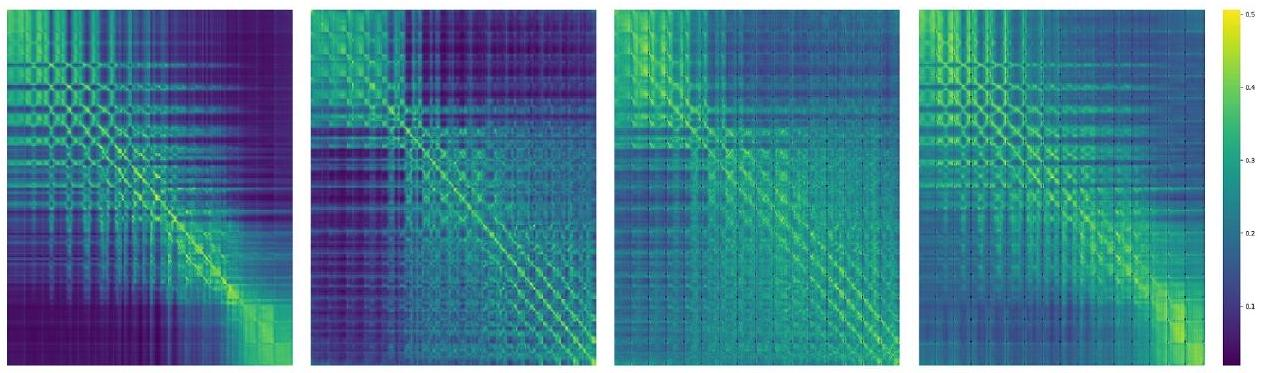
\includegraphics[width=\textwidth]{2025_10_26_62f95e615e8879e267a8g-12}
\captionsetup{labelformat=empty}
\caption{Figure 9: Token dependency plotted. The normalized heat map of attention scores in the last self-attention layer of VQGAN encoder is visualized. 4 random $256 \times 256$ images from ImageNet validation set are used.}
\end{center}
\end{figure}

\section*{A Token dependency in VQVAE}
To examine the token dependency in VQVAE [30], we check the attention scores in the self-attention layer before the vector quantization module. We randomly sample $4256 \times 256$ images from the ImageNet validation set for this analysis. Note the self-attention layer in [30] only has 1 head so for each image we just plot one attention map. The heat map in Fig. 9 shows the attention scores of each token to all other tokens, which indicate a strong, bidirectional dependency among all tokens. This is not surprising since the VQVAE model, trained to reconstruct images, leverages self-attention layers without any attention mask. Some work [86] has used causal attention in self-attention layers of a video VAE, but we did not find any image VAE work uses causal self-attention.

\section*{B Time complexity of AR and VAR generation}
We prove the time complexity of AR and VAR generation.\\
Lemma B.1 For a standard self-attention transformer, the time complexity of $A R$ generation is $\mathcal{O}\left(n^{6}\right)$, where $h=w=n$ and $h, w$ are the height and width of the VQ code map, respectively.

Proof. The total number of tokens is $h \times w=n^{2}$. For the $i$-th ( $1 \leq i \leq n^{2}$ ) autoregressive iteration, the attention scores between each token and all other tokens need to be computed, which requires $\mathcal{O}\left(i^{2}\right)$ time. So the total time complexity would be:

$$
\sum_{i=1}^{n^{2}} i^{2}=\frac{1}{6} n^{2}\left(n^{2}+1\right)\left(2 n^{2}+1\right)
$$

Which is equivalent to $\mathcal{O}\left(n^{6}\right)$ basic computation.\\
For VAR, it needs us to define the resolution sequense ( $h_{1}, w_{1}, h_{2}, w_{2}, \ldots, h_{K}, w_{K}$ ) for autoregressive generation, where $h_{i}, w_{i}$ are the height and width of the VQ code map at the $i$-th autoregressive step, and $h_{K}=h, w_{K}=w$ reaches the final resolution. Suppose $n_{k}=h_{k}=w_{k}$ for all $1 \leq k \leq K$ and $n=h=w$, for simplicity. We set the resolutions as $n_{k}=a^{(k-1)}$ where $a>1$ is a constant such that $a^{(K-1)}=n$.\\
Lemma B.2. For a standard self-attention transformer and given hyperparameter $a>1$, the time complexity of VAR generation is $\mathcal{O}\left(n^{4}\right)$, where $h=w=n$ and $h, w$ are the height and width of the last (largest) VQ code map, respectively.

Proof. Consider the $k$-th ( $1 \leq k \leq K$ ) autoregressive generation. The total number of tokens of current all token maps ( $r_{1}, r_{2}, \ldots, r_{k}$ ) is:

$$
\sum_{i=1}^{k} n_{i}^{2}=\sum_{i=1}^{k} a^{2 \cdot(k-1)}=\frac{a^{2 k}-1}{a^{2}-1} .
$$

So the time complexity of the $k$-th autoregressive generation would be:

$$
\left(\frac{a^{2 k}-1}{a^{2}-1}\right)^{2}
$$

By summing up all autoregressive generations, we have:

$$
\begin{aligned}
& \sum_{k=1}^{\log _{a}(n)+1}\left(\frac{a^{2 k}-1}{a^{2}-1}\right)^{2} \\
& =\frac{\left(a^{4}-1\right) \log n+\left(a^{8} n^{4}-2 a^{6} n^{2}-2 a^{4}\left(n^{2}-1\right)+2 a^{2}-1\right) \log a}{\left(a^{2}-1\right)^{3}\left(a^{2}+1\right) \log a} \\
& \sim \mathcal{O}\left(n^{4}\right) .
\end{aligned}
$$

This completes the proof.

\begin{figure}[h]
\begin{center}
  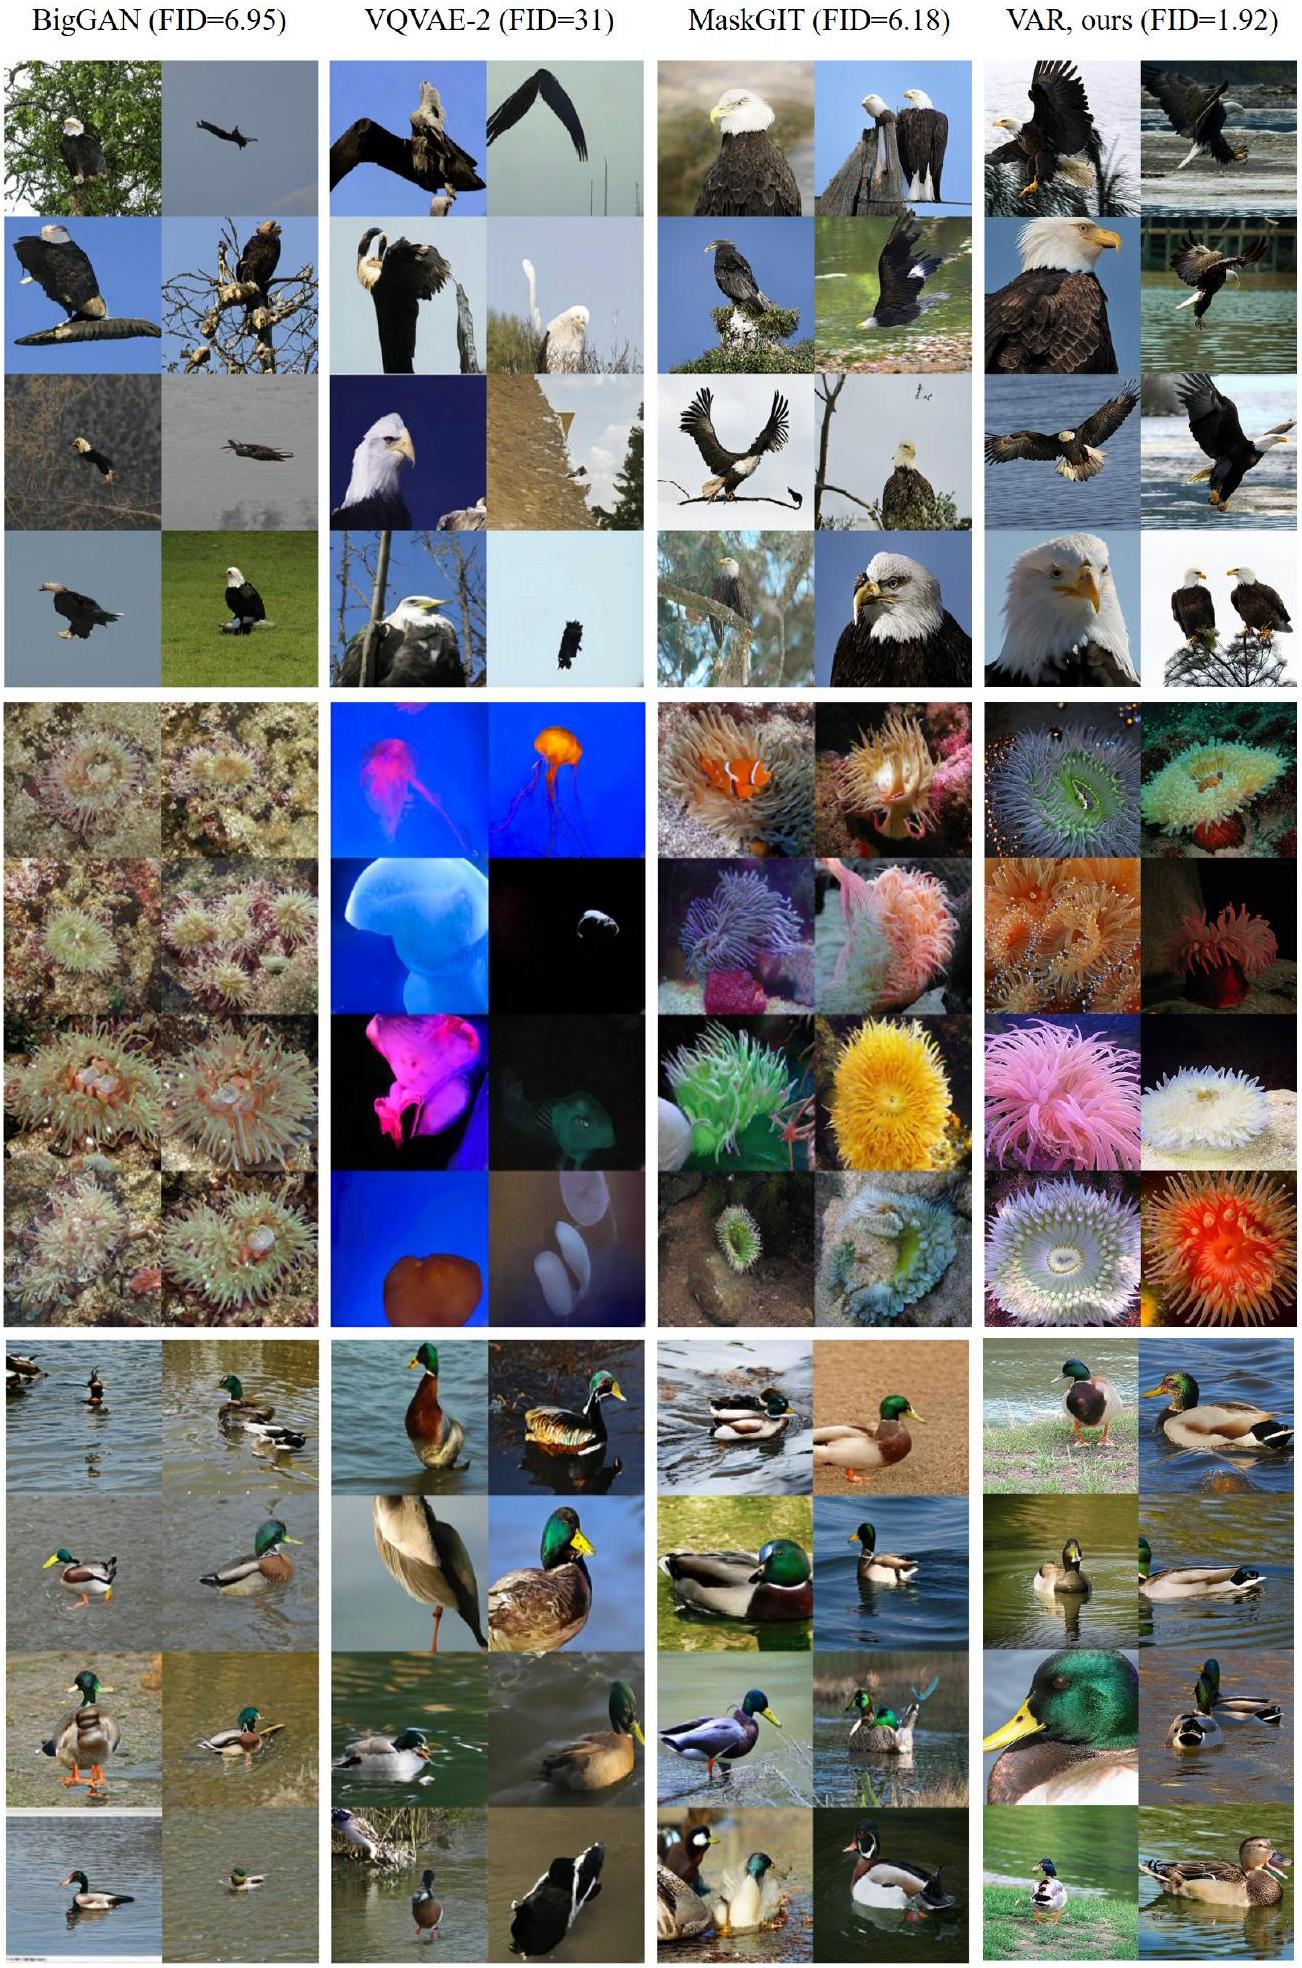
\includegraphics[width=\textwidth]{2025_10_26_62f95e615e8879e267a8g-14}
\captionsetup{labelformat=empty}
\caption{Figure 10: Model comparison on ImageNet \$\textbackslash mathbf\{2 5 6} \textbackslash times \textbackslash mathbf\{2 5 6\}\$ benchmark. More generated $512 \times 512$ samples by VAR can be found in the submitted Supplementary Material zip file.\}\end{center}
\end{figure}

\begin{figure}[h]
\begin{center}
  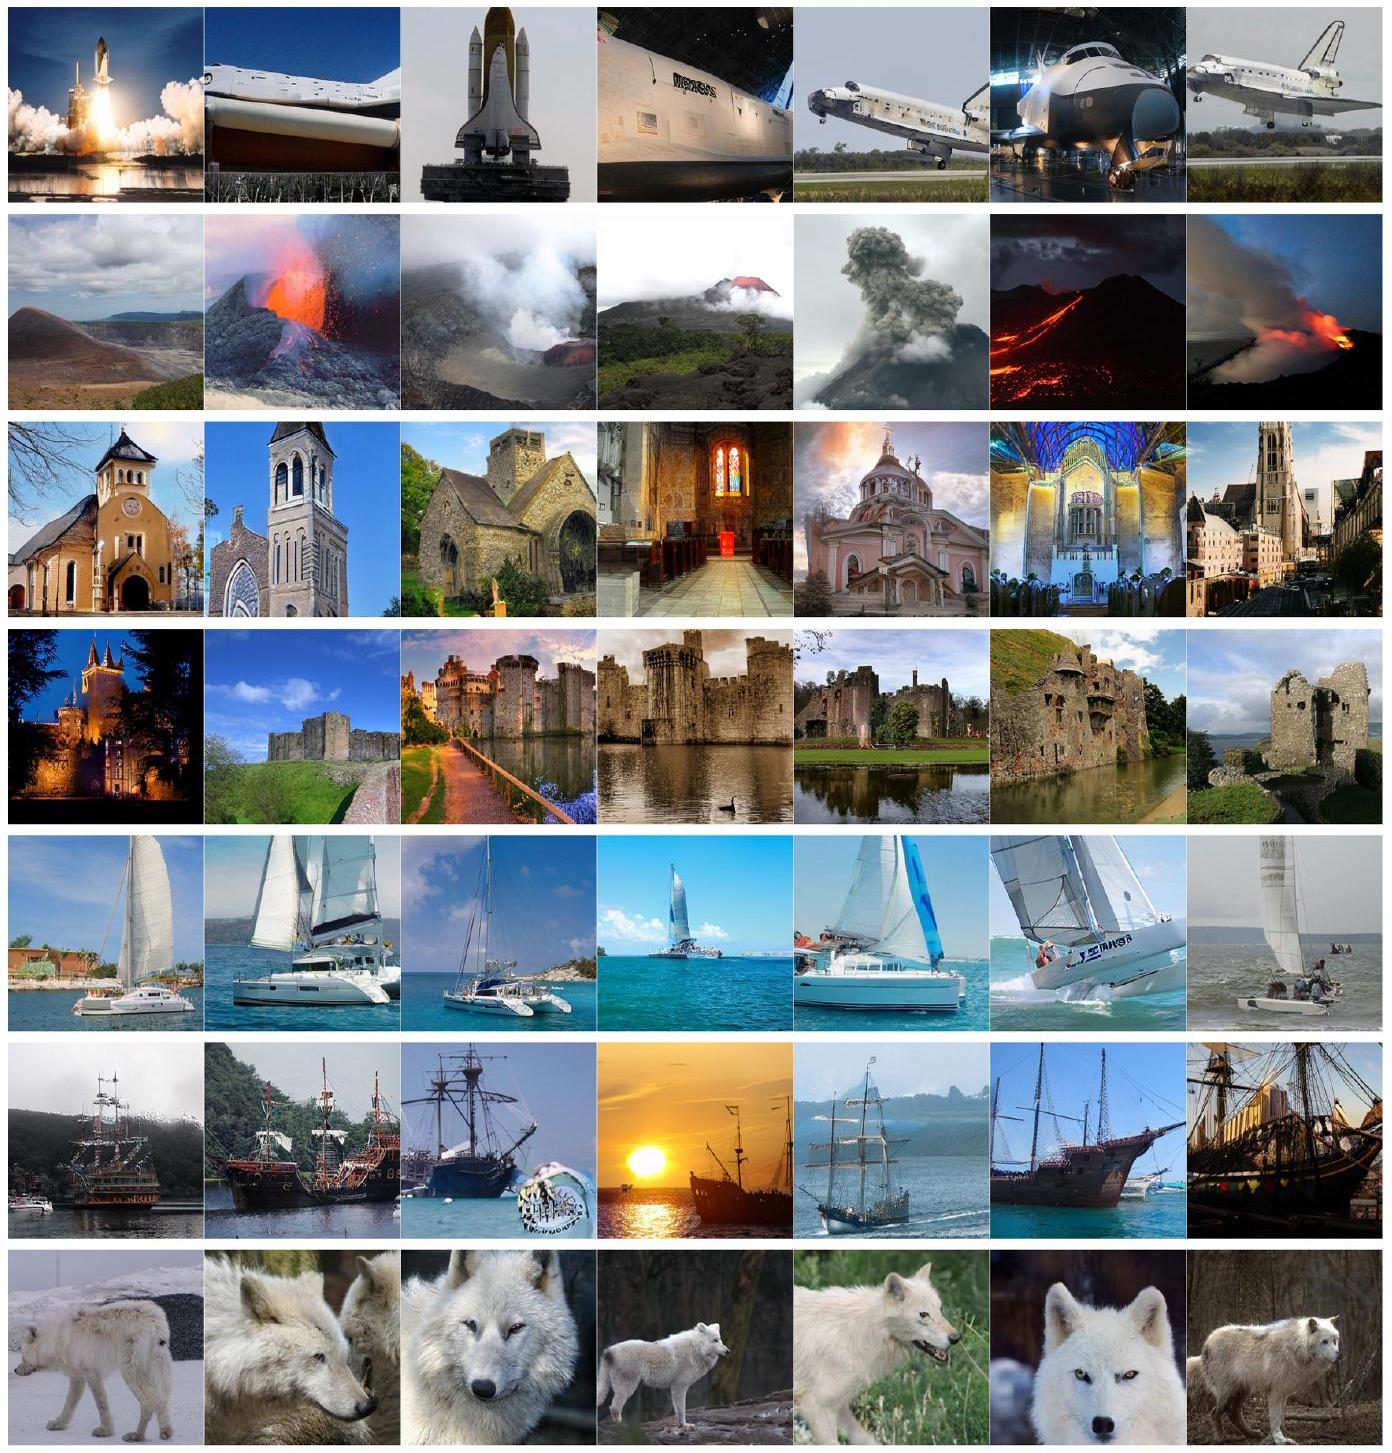
\includegraphics[width=\textwidth]{2025_10_26_62f95e615e8879e267a8g-15}
\captionsetup{labelformat=empty}
\caption{Figure 11: Some generated \$\textbackslash mathbf\{2 5 6} \textbackslash boldsymbol\{\textbackslash times\} \textbackslash mathbf\{2 5 6\}\$ samples by VAR trained on ImageNet. More generated $\mathbf{5 1 2 \times 5 1 2}$ samples by VAR can be found in the submitted Supplementary Material zip file.\}\end{center}
\end{figure}

\section*{References}
[1] J. Achiam, S. Adler, S. Agarwal, L. Ahmad, I. Akkaya, F. L. Aleman, D. Almeida, J. Altenschmidt, S. Altman, S. Anadkat, et al. Gpt-4 technical report. arXiv preprint arXiv:2303.08774, 2023. 2, 3, 8, 9\\[0pt]
[2] J.-B. Alayrac, J. Donahue, P. Luc, A. Miech, I. Barr, Y. Hasson, K. Lenc, A. Mensch, K. Millican, M. Reynolds, et al. Flamingo: a visual language model for few-shot learning. Advances in neural information processing systems, 35:23716-23736, 2022. 3\\[0pt]
[3] Alpha-VLLM. Large-dit-imagenet. \href{https://github.com/Alpha-VLLM/LLaMA2-Accessory/tree/}{https://github.com/Alpha-VLLM/LLaMA2-Accessory/tree/} f7fe19834b23e38f333403b91bb0330afe19f79e/Large-DiT-ImageNet, 2024. 2, 7, 8\\[0pt]
[4] R. Anil, A. M. Dai, O. Firat, M. Johnson, D. Lepikhin, A. Passos, S. Shakeri, E. Taropa, P. Bailey, Z. Chen, et al. Palm 2 technical report. arXiv preprint arXiv:2305.10403, 2023. 2\\[0pt]
[5] J. Bai, S. Bai, Y. Chu, Z. Cui, K. Dang, X. Deng, Y. Fan, W. Ge, Y. Han, F. Huang, et al. Qwen technical report. arXiv preprint arXiv:2309.16609, 2023. 2\\[0pt]
[6] Y. Bai, X. Geng, K. Mangalam, A. Bar, A. Yuille, T. Darrell, J. Malik, and A. A. Efros. Sequential modeling enables scalable learning for large vision models. arXiv preprint arXiv:2312.00785, 2023. 2, 3\\[0pt]
[7] F. Bao, C. Li, J. Zhu, and B. Zhang. Analytic-dpm: an analytic estimate of the optimal reverse variance in diffusion probabilistic models. arXiv preprint arXiv:2201.06503, 2022. 3\\[0pt]
[8] F. Bao, S. Nie, K. Xue, Y. Cao, C. Li, H. Su, and J. Zhu. All are worth words: A vit backbone for diffusion models. In Proceedings of the IEEE/CVF Conference on Computer Vision and Pattern Recognition, pages 22669-22679, 2023. 3\\[0pt]
[9] F. Bao, C. Xiang, G. Yue, G. He, H. Zhu, K. Zheng, M. Zhao, S. Liu, Y. Wang, and J. Zhu. Vidu: a highly consistent, dynamic and skilled text-to-video generator with diffusion models. arXiv preprint arXiv:2405.04233, 2024. 3\\[0pt]
[10] H. Bao, L. Dong, S. Piao, and F. Wei. Beit: Bert pre-training of image transformers. arXiv preprint arXiv:2106.08254, 2021. 3\\[0pt]
[11] A. Bar, Y. Gandelsman, T. Darrell, A. Globerson, and A. Efros. Visual prompting via image inpainting. Advances in Neural Information Processing Systems, 35:25005-25017, 2022. 3\\[0pt]
[12] O. Bar-Tal, H. Chefer, O. Tov, C. Herrmann, R. Paiss, S. Zada, A. Ephrat, J. Hur, Y. Li, T. Michaeli, et al. Lumiere: A space-time diffusion model for video generation. arXiv preprint arXiv:2401.12945, 2024. 3\\[0pt]
[13] A. Brock, J. Donahue, and K. Simonyan. Large scale gan training for high fidelity natural image synthesis. arXiv preprint arXiv:1809.11096, 2018. 7\\[0pt]
[14] T. Brooks, B. Peebles, C. Holmes, W. DePue, Y. Guo, L. Jing, D. Schnurr, J. Taylor, T. Luhman, E. Luhman, C. Ng, R. Wang, and A. Ramesh. Video generation models as world simulators. OpenAI, 2024. 3, 7, 12\\[0pt]
[15] T. Brown, B. Mann, N. Ryder, M. Subbiah, J. D. Kaplan, P. Dhariwal, A. Neelakantan, P. Shyam, G. Sastry, A. Askell, et al. Language models are few-shot learners. Advances in neural information processing systems, 33:1877-1901, 2020. 2, 3\\[0pt]
[16] H. Chang, H. Zhang, J. Barber, A. Maschinot, J. Lezama, L. Jiang, M.-H. Yang, K. Murphy, W. T. Freeman, M. Rubinstein, et al. Muse: Text-to-image generation via masked generative transformers. arXiv preprint arXiv:2301.00704, 2023. 3\\[0pt]
[17] H. Chang, H. Zhang, L. Jiang, C. Liu, and W. T. Freeman. Maskgit: Masked generative image transformer. In Proceedings of the IEEE/CVF Conference on Computer Vision and Pattern Recognition, pages 1131511325, 2022. 3, 7, 10, 11\\[0pt]
[18] J. Chen, C. Ge, E. Xie, Y. Wu, L. Yao, X. Ren, Z. Wang, P. Luo, H. Lu, and Z. Li. Pixart- $\backslash$ sigma: Weak-tostrong training of diffusion transformer for 4k text-to-image generation. arXiv preprint arXiv:2403.04692, 2024. 3\\[0pt]
[19] J. Chen, J. Yu, C. Ge, L. Yao, E. Xie, Y. Wu, Z. Wang, J. Kwok, P. Luo, H. Lu, et al. Pixart: Fast training of diffusion transformer for photorealistic text-to-image synthesis. arXiv preprint arXiv:2310.00426, 2023. 3, 6\\[0pt]
[20] M. Chen, A. Radford, R. Child, J. Wu, H. Jun, D. Luan, and I. Sutskever. Generative pretraining from pixels. In International conference on machine learning, pages 1691-1703. PMLR, 2020. 3\\[0pt]
[21] Z. Chen, J. Wu, W. Wang, W. Su, G. Chen, S. Xing, Z. Muyan, Q. Zhang, X. Zhu, L. Lu, et al. Internvl: Scaling up vision foundation models and aligning for generic visual-linguistic tasks. arXiv preprint arXiv:2312.14238, 2023. 3\\[0pt]
[22] A. Chowdhery, S. Narang, J. Devlin, M. Bosma, G. Mishra, A. Roberts, P. Barham, H. W. Chung, C. Sutton, S. Gehrmann, et al. Palm: Scaling language modeling with pathways. Journal of Machine Learning Research, 24(240):1-113, 2023. 2\\[0pt]
[23] X. Dai, J. Hou, C.-Y. Ma, S. Tsai, J. Wang, R. Wang, P. Zhang, S. Vandenhende, X. Wang, A. Dubey, et al. Emu: Enhancing image generation models using photogenic needles in a haystack. arXiv preprint arXiv:2309.15807, 2023. 3\\[0pt]
[24] J. Deng, W. Dong, R. Socher, L.-J. Li, K. Li, and L. Fei-Fei. Imagenet: A large-scale hierarchical image database. In 2009 IEEE conference on computer vision and pattern recognition, pages 248-255. Ieee, 2009. 8\\[0pt]
[25] J. Devlin, M.-W. Chang, K. Lee, and K. Toutanova. Bert: Pre-training of deep bidirectional transformers for language understanding. arXiv preprint arXiv:1810.04805, 2018. 3\\[0pt]
[26] P. Dhariwal and A. Nichol. Diffusion models beat gans on image synthesis. Advances in neural information processing systems, 34:8780-8794, 2021. 7\\[0pt]
[27] R. Dong, C. Han, Y. Peng, Z. Qi, Z. Ge, J. Yang, L. Zhao, J. Sun, H. Zhou, H. Wei, et al. Dreamllm: Synergistic multimodal comprehension and creation. arXiv preprint arXiv:2309.11499, 2023. 3\\[0pt]
[28] A. Dosovitskiy, L. Beyer, A. Kolesnikov, D. Weissenborn, X. Zhai, T. Unterthiner, M. Dehghani, M. Minderer, G. Heigold, S. Gelly, et al. An image is worth $16 \times 16$ words: Transformers for image recognition at scale. arXiv preprint arXiv:2010.11929, 2020. 3\\[0pt]
[29] P. Esser, S. Kulal, A. Blattmann, R. Entezari, J. Müller, H. Saini, Y. Levi, D. Lorenz, A. Sauer, F. Boesel, D. Podell, T. Dockhorn, Z. English, K. Lacey, A. Goodwin, Y. Marek, and R. Rombach. Scaling rectified flow transformers for high-resolution image synthesis, 2024. 3, 7\\[0pt]
[30] P. Esser, R. Rombach, and B. Ommer. Taming transformers for high-resolution image synthesis. In Proceedings of the IEEE/CVF conference on computer vision and pattern recognition, pages 12873-12883, 2021. 2, 3, 4, 5, 6, 7, 11, 12, 13\\[0pt]
[31] Y. Ge, S. Zhao, Z. Zeng, Y. Ge, C. Li, X. Wang, and Y. Shan. Making llama see and draw with seed tokenizer. arXiv preprint arXiv:2310.01218, 2023. 3\\[0pt]
[32] Y. Ge, S. Zhao, J. Zhu, Y. Ge, K. Yi, L. Song, C. Li, X. Ding, and Y. Shan. Seed-x: Multimodal models with unified multi-granularity comprehension and generation. arXiv preprint arXiv:2404.14396, 2024. 3\\[0pt]
[33] A. Gupta, L. Yu, K. Sohn, X. Gu, M. Hahn, L. Fei-Fei, I. Essa, L. Jiang, and J. Lezama. Photorealistic video generation with diffusion models. arXiv preprint arXiv:2312.06662, 2023. 3\\[0pt]
[34] K. He, X. Chen, S. Xie, Y. Li, P. Dollár, and R. Girshick. Masked autoencoders are scalable vision learners. In Proceedings of the IEEE/CVF conference on computer vision and pattern recognition, pages 16000-16009, 2022. 3\\[0pt]
[35] T. Henighan, J. Kaplan, M. Katz, M. Chen, C. Hesse, J. Jackson, H. Jun, T. B. Brown, P. Dhariwal, S. Gray, et al. Scaling laws for autoregressive generative modeling. arXiv preprint arXiv:2010.14701, 2020. 2, 3, 8, 9\\[0pt]
[36] J. Ho, C. Saharia, W. Chan, D. J. Fleet, M. Norouzi, and T. Salimans. Cascaded diffusion models for high fidelity image generation. The Journal of Machine Learning Research, 23(1):2249-2281, 2022. 3, 7\\[0pt]
[37] J. Ho and T. Salimans. Classifier-free diffusion guidance. arXiv preprint arXiv:2207.12598, 2022. 3\\[0pt]
[38] J. Hoffmann, S. Borgeaud, A. Mensch, E. Buchatskaya, T. Cai, E. Rutherford, D. d. L. Casas, L. A. Hendricks, J. Welbl, A. Clark, et al. Training compute-optimal large language models. arXiv preprint arXiv:2203.15556, 2022. 2, 3, 8, 9\\[0pt]
[39] L. Huang, W. Yu, W. Ma, W. Zhong, Z. Feng, H. Wang, Q. Chen, W. Peng, X. Feng, B. Qin, et al. A survey on hallucination in large language models: Principles, taxonomy, challenges, and open questions. arXiv preprint arXiv:2311.05232, 2023. 2\\[0pt]
[40] M. Jia, L. Tang, B.-C. Chen, C. Cardie, S. Belongie, B. Hariharan, and S.-N. Lim. Visual prompt tuning. In European Conference on Computer Vision, pages 709-727. Springer, 2022. 3\\[0pt]
[41] Y. Jin, K. Xu, L. Chen, C. Liao, J. Tan, B. Chen, C. Lei, A. Liu, C. Song, X. Lei, et al. Unified languagevision pretraining with dynamic discrete visual tokenization. arXiv preprint arXiv:2309.04669, 2023. 3\\[0pt]
[42] M. Kang, J.-Y. Zhu, R. Zhang, J. Park, E. Shechtman, S. Paris, and T. Park. Scaling up gans for text-toimage synthesis. In Proceedings of the IEEE/CVF Conference on Computer Vision and Pattern Recognition, pages 10124-10134, 2023. 6, 7\\[0pt]
[43] J. Kaplan, S. McCandlish, T. Henighan, T. B. Brown, B. Chess, R. Child, S. Gray, A. Radford, J. Wu, and D. Amodei. Scaling laws for neural language models. arXiv preprint arXiv:2001.08361, 2020. 2, 3, 6, 8, 9\\[0pt]
[44] T. Karras, T. Aila, S. Laine, and J. Lehtinen. Progressive growing of gans for improved quality, stability, and variation. arXiv preprint arXiv:1710.10196, 2017. 2\\[0pt]
[45] T. Karras, M. Aittala, S. Laine, E. Härkönen, J. Hellsten, J. Lehtinen, and T. Aila. Alias-free generative adversarial networks. Advances in Neural Information Processing Systems, 34:852-863, 2021. 6\\[0pt]
[46] T. Karras, S. Laine, and T. Aila. A style-based generator architecture for generative adversarial networks. In Proceedings of the IEEE/CVF conference on computer vision and pattern recognition, pages 4401-4410, 2019. 4, 6\\[0pt]
[47] T. Karras, S. Laine, M. Aittala, J. Hellsten, J. Lehtinen, and T. Aila. Analyzing and improving the image quality of stylegan. In Proceedings of the IEEE/CVF conference on computer vision and pattern recognition, pages 8110-8119, 2020. 6\\[0pt]
[48] A. Kirillov, E. Mintun, N. Ravi, H. Mao, C. Rolland, L. Gustafson, T. Xiao, S. Whitehead, A. C. Berg, W.-Y. Lo, et al. Segment anything. arXiv preprint arXiv:2304.02643, 2023. 3\\[0pt]
[49] A. Kuznetsova, H. Rom, N. Alldrin, J. Uijlings, I. Krasin, J. Pont-Tuset, S. Kamali, S. Popov, M. Malloci, A. Kolesnikov, et al. The open images dataset v4: Unified image classification, object detection, and visual relationship detection at scale. International Journal of Computer Vision, 128(7):1956-1981, 2020. 6\\[0pt]
[50] D. Lee, C. Kim, S. Kim, M. Cho, and W.-S. Han. Autoregressive image generation using residual quantization. In Proceedings of the IEEE/CVF Conference on Computer Vision and Pattern Recognition, pages 11523-11532, 2022. 2, 3, 4, 5, 6, 7\\[0pt]
[51] T. Li, D. Katabi, and K. He. Self-conditioned image generation via generating representations. arXiv preprint arXiv:2312.03701, 2023. 2, 7\\[0pt]
[52] T.-Y. Lin, P. Dollár, R. Girshick, K. He, B. Hariharan, and S. Belongie. Feature pyramid networks for object detection. In Proceedings of the IEEE conference on computer vision and pattern recognition, pages 2117-2125, 2017. 2\\[0pt]
[53] H. Liu, C. Li, Q. Wu, and Y. J. Lee. Visual instruction tuning. Advances in neural information processing systems, 36, 2024. 3\\[0pt]
[54] D. G. Lowe. Object recognition from local scale-invariant features. In Proceedings of the seventh IEEE international conference on computer vision, volume 2, pages 1150-1157. Ieee, 1999. 2\\[0pt]
[55] C. Lu, Y. Zhou, F. Bao, J. Chen, C. Li, and J. Zhu. Dpm-solver: A fast ode solver for diffusion probabilistic model sampling in around 10 steps. Advances in Neural Information Processing Systems, 35:5775-5787, 2022. 3\\[0pt]
[56] C. Lu, Y. Zhou, F. Bao, J. Chen, C. Li, and J. Zhu. Dpm-solver++: Fast solver for guided sampling of diffusion probabilistic models. arXiv preprint arXiv:2211.01095, 2022. 3\\[0pt]
[57] J. Lu, C. Clark, S. Lee, Z. Zhang, S. Khosla, R. Marten, D. Hoiem, and A. Kembhavi. Unified-io 2: Scaling autoregressive multimodal models with vision, language, audio, and action. arXiv preprint arXiv:2312.17172, 2023. 2\\[0pt]
[58] J. Lu, C. Clark, R. Zellers, R. Mottaghi, and A. Kembhavi. Unified-io: A unified model for vision, language, and multi-modal tasks. arXiv preprint arXiv:2206.08916, 2022. 2\\[0pt]
[59] F. Mentzer, D. Minnen, E. Agustsson, and M. Tschannen. Finite scalar quantization: Vq-vae made simple. arXiv preprint arXiv:2309.15505, 2023. 12\\[0pt]
[60] A. Nichol, P. Dhariwal, A. Ramesh, P. Shyam, P. Mishkin, B. McGrew, I. Sutskever, and M. Chen. Glide: Towards photorealistic image generation and editing with text-guided diffusion models. arXiv preprint arXiv:2112.10741, 2021. 3\\[0pt]
[61] M. Oquab, T. Darcet, T. Moutakanni, H. Vo, M. Szafraniec, V. Khalidov, P. Fernandez, D. Haziza, F. Massa, A. El-Nouby, et al. Dinov2: Learning robust visual features without supervision. arXiv preprint arXiv:2304.07193, 2023. 3\\[0pt]
[62] L. Ouyang, J. Wu, X. Jiang, D. Almeida, C. Wainwright, P. Mishkin, C. Zhang, S. Agarwal, K. Slama, A. Ray, et al. Training language models to follow instructions with human feedback. Advances in Neural Information Processing Systems, 35:27730-27744, 2022. 2\\[0pt]
[63] W. Peebles and S. Xie. Scalable diffusion models with transformers. In Proceedings of the IEEE/CVF International Conference on Computer Vision, pages 4195-4205, 2023. 2, 3, 6, 7, 8\\[0pt]
[64] A. Radford, J. W. Kim, C. Hallacy, A. Ramesh, G. Goh, S. Agarwal, G. Sastry, A. Askell, P. Mishkin, J. Clark, et al. Learning transferable visual models from natural language supervision. In International conference on machine learning, pages 8748-8763. PMLR, 2021. 3\\[0pt]
[65] A. Radford, K. Narasimhan, T. Salimans, I. Sutskever, et al. Improving language understanding by generative pre-training. article, 2018. 2\\[0pt]
[66] A. Radford, J. Wu, R. Child, D. Luan, D. Amodei, I. Sutskever, et al. Language models are unsupervised multitask learners. OpenAI blog, 1(8):9, 2019. 2, 3, 6\\[0pt]
[67] A. Ramesh, M. Pavlov, G. Goh, S. Gray, C. Voss, A. Radford, M. Chen, and I. Sutskever. Zero-shot text-to-image generation. In International Conference on Machine Learning, pages 8821-8831. PMLR, 2021. 2\\[0pt]
[68] A. Razavi, A. Van den Oord, and O. Vinyals. Generating diverse high-fidelity images with vq-vae-2. Advances in neural information processing systems, 32, 2019. 2, 3, 7\\[0pt]
[69] S. Reed, A. Oord, N. Kalchbrenner, S. G. Colmenarejo, Z. Wang, Y. Chen, D. Belov, and N. Freitas. Parallel multiscale autoregressive density estimation. In International conference on machine learning, pages 2912-2921. PMLR, 2017. 3\\[0pt]
[70] R. Rombach, A. Blattmann, D. Lorenz, P. Esser, and B. Ommer. High-resolution image synthesis with latent diffusion models. In Proceedings of the IEEE/CVF conference on computer vision and pattern recognition, pages 10684-10695, 2022. 3, 7\\[0pt]
[71] C. Saharia, W. Chan, S. Saxena, L. Li, J. Whang, E. L. Denton, K. Ghasemipour, R. Gontijo Lopes, B. Karagol Ayan, T. Salimans, et al. Photorealistic text-to-image diffusion models with deep language understanding. Advances in Neural Information Processing Systems, 35:36479-36494, 2022. 3\\[0pt]
[72] V. Sanh, A. Webson, C. Raffel, S. H. Bach, L. Sutawika, Z. Alyafeai, A. Chaffin, A. Stiegler, T. L. Scao, A. Raja, et al. Multitask prompted training enables zero-shot task generalization. arXiv preprint arXiv:2110.08207, 2021. 3\\[0pt]
[73] A. Sauer, T. Karras, S. Laine, A. Geiger, and T. Aila. Stylegan-t: Unlocking the power of gans for fast large-scale text-to-image synthesis. arXiv preprint arXiv:2301.09515, 2023. 6\\[0pt]
[74] A. Sauer, K. Schwarz, and A. Geiger. Stylegan-xl: Scaling stylegan to large diverse datasets. In ACM SIGGRAPH 2022 conference proceedings, pages 1-10, 2022. 6, 7\\[0pt]
[75] J. Song, C. Meng, and S. Ermon. Denoising diffusion implicit models. arXiv preprint arXiv:2010.02502, 2020. 3\\[0pt]
[76] Y. Song and S. Ermon. Generative modeling by estimating gradients of the data distribution. Advances in neural information processing systems, 32, 2019. 3\\[0pt]
[77] Q. Sun, Q. Yu, Y. Cui, F. Zhang, X. Zhang, Y. Wang, H. Gao, J. Liu, T. Huang, and X. Wang. Generative pretraining in multimodality. arXiv preprint arXiv:2307.05222, 2023. 3\\[0pt]
[78] Y. Sun, S. Wang, S. Feng, S. Ding, C. Pang, J. Shang, J. Liu, X. Chen, Y. Zhao, Y. Lu, et al. Ernie 3.0: Large-scale knowledge enhanced pre-training for language understanding and generation. arXiv preprint arXiv:2107.02137, 2021. 2\\[0pt]
[79] G. Team, R. Anil, S. Borgeaud, Y. Wu, J.-B. Alayrac, J. Yu, R. Soricut, J. Schalkwyk, A. M. Dai, A. Hauth, et al. Gemini: a family of highly capable multimodal models. arXiv preprint arXiv:2312.11805, 2023. 2\\[0pt]
[80] C. Tian, X. Zhu, Y. Xiong, W. Wang, Z. Chen, W. Wang, Y. Chen, L. Lu, T. Lu, J. Zhou, et al. Mminterleaved: Interleaved image-text generative modeling via multi-modal feature synchronizer. arXiv preprint arXiv:2401.10208, 2024. 3\\[0pt]
[81] K. Tian, Y. Jiang, Q. Diao, C. Lin, L. Wang, and Z. Yuan. Designing bert for convolutional networks: Sparse and hierarchical masked modeling. arXiv preprint arXiv:2301.03580, 2023. 2\\[0pt]
[82] H. Touvron, T. Lavril, G. Izacard, X. Martinet, M.-A. Lachaux, T. Lacroix, B. Rozière, N. Goyal, E. Hambro, F. Azhar, et al. Llama: Open and efficient foundation language models. arXiv preprint arXiv:2302.13971, 2023. 2, 3, 6\\[0pt]
[83] H. Touvron, L. Martin, K. Stone, P. Albert, A. Almahairi, Y. Babaei, N. Bashlykov, S. Batra, P. Bhargava, S. Bhosale, et al. Llama 2: Open foundation and fine-tuned chat models. arXiv preprint arXiv:2307.09288, 2023. 2, 3, 6\\[0pt]
[84] A. Van den Oord, N. Kalchbrenner, L. Espeholt, O. Vinyals, A. Graves, et al. Conditional image generation with pixelcnn decoders. Advances in neural information processing systems, 29, 2016. 3\\[0pt]
[85] A. Van Den Oord, O. Vinyals, et al. Neural discrete representation learning. Advances in neural information processing systems, 30, 2017. 3\\[0pt]
[86] R. Villegas, M. Babaeizadeh, P.-J. Kindermans, H. Moraldo, H. Zhang, M. T. Saffar, S. Castro, J. Kunze, and D. Erhan. Phenaki: Variable length video generation from open domain textual descriptions. In International Conference on Learning Representations, 2022. 13\\[0pt]
[87] H. Wang, H. Tang, L. Jiang, S. Shi, M. F. Naeem, H. Li, B. Schiele, and L. Wang. Git: Towards generalist vision transformer through universal language interface. arXiv preprint arXiv:2403.09394, 2024. 3\\[0pt]
[88] W. Wang, Z. Chen, X. Chen, J. Wu, X. Zhu, G. Zeng, P. Luo, T. Lu, J. Zhou, Y. Qiao, et al. Visionllm: Large language model is also an open-ended decoder for vision-centric tasks. Advances in Neural Information Processing Systems, 36, 2024. 3\\[0pt]
[89] X. Wang, W. Wang, Y. Cao, C. Shen, and T. Huang. Images speak in images: A generalist painter for in-context visual learning. In Proceedings of the IEEE/CVF Conference on Computer Vision and Pattern Recognition, pages 6830-6839, 2023. 3\\[0pt]
[90] B. Workshop, T. L. Scao, A. Fan, C. Akiki, E. Pavlick, S. Ilić, D. Hesslow, R. Castagné, A. S. Luccioni, F. Yvon, et al. Bloom: A 176b-parameter open-access multilingual language model. arXiv preprint arXiv:2211.05100, 2022. 2, 3\\[0pt]
[91] Z. Xue, G. Song, Q. Guo, B. Liu, Z. Zong, Y. Liu, and P. Luo. Raphael: Text-to-image generation via large mixture of diffusion paths. arXiv preprint arXiv:2305.18295, 2023. 3\\[0pt]
[92] J. Yu, X. Li, J. Y. Koh, H. Zhang, R. Pang, J. Qin, A. Ku, Y. Xu, J. Baldridge, and Y. Wu. Vector-quantized image modeling with improved vqgan. arXiv preprint arXiv:2110.04627, 2021. 2, 3, 4, 6, 7\\[0pt]
[93] J. Yu, Y. Xu, J. Y. Koh, T. Luong, G. Baid, Z. Wang, V. Vasudevan, A. Ku, Y. Yang, B. K. Ayan, et al. Scaling autoregressive models for content-rich text-to-image generation. arXiv preprint arXiv:2206.10789, 2(3):5, 2022. 3\\[0pt]
[94] L. Yu, Y. Cheng, K. Sohn, J. Lezama, H. Zhang, H. Chang, A. G. Hauptmann, M.-H. Yang, Y. Hao, I. Essa, et al. Magvit: Masked generative video transformer. In Proceedings of the IEEE/CVF Conference on Computer Vision and Pattern Recognition, pages 10459-10469, 2023. 3\\[0pt]
[95] L. Yu, J. Lezama, N. B. Gundavarapu, L. Versari, K. Sohn, D. Minnen, Y. Cheng, A. Gupta, X. Gu, A. G. Hauptmann, et al. Language model beats diffusion-tokenizer is key to visual generation. arXiv preprint arXiv:2310.05737, 2023. 3, 12\\[0pt]
[96] L. Yu, B. Shi, R. Pasunuru, B. Muller, O. Golovneva, T. Wang, A. Babu, B. Tang, B. Karrer, S. Sheynin, et al. Scaling autoregressive multi-modal models: Pretraining and instruction tuning. arXiv preprint arXiv:2309.02591, 2(3), 2023. 3\\[0pt]
[97] R. Zhang, P. Isola, A. A. Efros, E. Shechtman, and O. Wang. The unreasonable effectiveness of deep features as a perceptual metric. In Proceedings of the IEEE conference on computer vision and pattern recognition, pages 586-595, 2018. 4\\[0pt]
[98] S. Zhang, S. Roller, N. Goyal, M. Artetxe, M. Chen, S. Chen, C. Dewan, M. Diab, X. Li, X. V. Lin, et al. Opt: Open pre-trained transformer language models. arXiv preprint arXiv:2205.01068, 2022. 3\\[0pt]
[99] C. Zheng, T.-L. Vuong, J. Cai, and D. Phung. Movq: Modulating quantized vectors for high-fidelity image generation. Advances in Neural Information Processing Systems, 35:23412-23425, 2022. 2, 12


\end{document}